\documentclass{article}
\usepackage{iclr2027_conference,times}
%%%%% NEW MATH DEFINITIONS %%%%%

\usepackage{amsmath,amsfonts,bm}

% Mark sections of captions for referring to divisions of figures
\newcommand{\figleft}{{\em (Left)}}
\newcommand{\figcenter}{{\em (Center)}}
\newcommand{\figright}{{\em (Right)}}
\newcommand{\figtop}{{\em (Top)}}
\newcommand{\figbottom}{{\em (Bottom)}}
\newcommand{\captiona}{{\em (a)}}
\newcommand{\captionb}{{\em (b)}}
\newcommand{\captionc}{{\em (c)}}
\newcommand{\captiond}{{\em (d)}}

% Highlight a newly defined term
\newcommand{\newterm}[1]{{\bf #1}}


% Figure reference, lower-case.
\def\figref#1{figure~\ref{#1}}
% Figure reference, capital. For start of sentence
\def\Figref#1{Figure~\ref{#1}}
\def\twofigref#1#2{figures \ref{#1} and \ref{#2}}
\def\quadfigref#1#2#3#4{figures \ref{#1}, \ref{#2}, \ref{#3} and \ref{#4}}
% Section reference, lower-case.
\def\secref#1{section~\ref{#1}}
% Section reference, capital.
\def\Secref#1{Section~\ref{#1}}
% Reference to two sections.
\def\twosecrefs#1#2{sections \ref{#1} and \ref{#2}}
% Reference to three sections.
\def\secrefs#1#2#3{sections \ref{#1}, \ref{#2} and \ref{#3}}
% Reference to an equation, lower-case.
\def\eqref#1{equation~\ref{#1}}
% Reference to an equation, upper case
\def\Eqref#1{Equation~\ref{#1}}
% A raw reference to an equation---avoid using if possible
\def\plaineqref#1{\ref{#1}}
% Reference to a chapter, lower-case.
\def\chapref#1{chapter~\ref{#1}}
% Reference to an equation, upper case.
\def\Chapref#1{Chapter~\ref{#1}}
% Reference to a range of chapters
\def\rangechapref#1#2{chapters\ref{#1}--\ref{#2}}
% Reference to an algorithm, lower-case.
\def\algref#1{algorithm~\ref{#1}}
% Reference to an algorithm, upper case.
\def\Algref#1{Algorithm~\ref{#1}}
\def\twoalgref#1#2{algorithms \ref{#1} and \ref{#2}}
\def\Twoalgref#1#2{Algorithms \ref{#1} and \ref{#2}}
% Reference to a part, lower case
\def\partref#1{part~\ref{#1}}
% Reference to a part, upper case
\def\Partref#1{Part~\ref{#1}}
\def\twopartref#1#2{parts \ref{#1} and \ref{#2}}

\def\ceil#1{\lceil #1 \rceil}
\def\floor#1{\lfloor #1 \rfloor}
\def\1{\bm{1}}
\newcommand{\train}{\mathcal{D}}
\newcommand{\valid}{\mathcal{D_{\mathrm{valid}}}}
\newcommand{\test}{\mathcal{D_{\mathrm{test}}}}

\def\eps{{\epsilon}}


% Random variables
\def\reta{{\textnormal{$\eta$}}}
\def\ra{{\textnormal{a}}}
\def\rb{{\textnormal{b}}}
\def\rc{{\textnormal{c}}}
\def\rd{{\textnormal{d}}}
\def\re{{\textnormal{e}}}
\def\rf{{\textnormal{f}}}
\def\rg{{\textnormal{g}}}
\def\rh{{\textnormal{h}}}
\def\ri{{\textnormal{i}}}
\def\rj{{\textnormal{j}}}
\def\rk{{\textnormal{k}}}
\def\rl{{\textnormal{l}}}
% rm is already a command, just don't name any random variables m
\def\rn{{\textnormal{n}}}
\def\ro{{\textnormal{o}}}
\def\rp{{\textnormal{p}}}
\def\rq{{\textnormal{q}}}
\def\rr{{\textnormal{r}}}
\def\rs{{\textnormal{s}}}
\def\rt{{\textnormal{t}}}
\def\ru{{\textnormal{u}}}
\def\rv{{\textnormal{v}}}
\def\rw{{\textnormal{w}}}
\def\rx{{\textnormal{x}}}
\def\ry{{\textnormal{y}}}
\def\rz{{\textnormal{z}}}

% Random vectors
\def\rvepsilon{{\mathbf{\epsilon}}}
\def\rvtheta{{\mathbf{\theta}}}
\def\rva{{\mathbf{a}}}
\def\rvb{{\mathbf{b}}}
\def\rvc{{\mathbf{c}}}
\def\rvd{{\mathbf{d}}}
\def\rve{{\mathbf{e}}}
\def\rvf{{\mathbf{f}}}
\def\rvg{{\mathbf{g}}}
\def\rvh{{\mathbf{h}}}
\def\rvu{{\mathbf{i}}}
\def\rvj{{\mathbf{j}}}
\def\rvk{{\mathbf{k}}}
\def\rvl{{\mathbf{l}}}
\def\rvm{{\mathbf{m}}}
\def\rvn{{\mathbf{n}}}
\def\rvo{{\mathbf{o}}}
\def\rvp{{\mathbf{p}}}
\def\rvq{{\mathbf{q}}}
\def\rvr{{\mathbf{r}}}
\def\rvs{{\mathbf{s}}}
\def\rvt{{\mathbf{t}}}
\def\rvu{{\mathbf{u}}}
\def\rvv{{\mathbf{v}}}
\def\rvw{{\mathbf{w}}}
\def\rvx{{\mathbf{x}}}
\def\rvy{{\mathbf{y}}}
\def\rvz{{\mathbf{z}}}

% Elements of random vectors
\def\erva{{\textnormal{a}}}
\def\ervb{{\textnormal{b}}}
\def\ervc{{\textnormal{c}}}
\def\ervd{{\textnormal{d}}}
\def\erve{{\textnormal{e}}}
\def\ervf{{\textnormal{f}}}
\def\ervg{{\textnormal{g}}}
\def\ervh{{\textnormal{h}}}
\def\ervi{{\textnormal{i}}}
\def\ervj{{\textnormal{j}}}
\def\ervk{{\textnormal{k}}}
\def\ervl{{\textnormal{l}}}
\def\ervm{{\textnormal{m}}}
\def\ervn{{\textnormal{n}}}
\def\ervo{{\textnormal{o}}}
\def\ervp{{\textnormal{p}}}
\def\ervq{{\textnormal{q}}}
\def\ervr{{\textnormal{r}}}
\def\ervs{{\textnormal{s}}}
\def\ervt{{\textnormal{t}}}
\def\ervu{{\textnormal{u}}}
\def\ervv{{\textnormal{v}}}
\def\ervw{{\textnormal{w}}}
\def\ervx{{\textnormal{x}}}
\def\ervy{{\textnormal{y}}}
\def\ervz{{\textnormal{z}}}

% Random matrices
\def\rmA{{\mathbf{A}}}
\def\rmB{{\mathbf{B}}}
\def\rmC{{\mathbf{C}}}
\def\rmD{{\mathbf{D}}}
\def\rmE{{\mathbf{E}}}
\def\rmF{{\mathbf{F}}}
\def\rmG{{\mathbf{G}}}
\def\rmH{{\mathbf{H}}}
\def\rmI{{\mathbf{I}}}
\def\rmJ{{\mathbf{J}}}
\def\rmK{{\mathbf{K}}}
\def\rmL{{\mathbf{L}}}
\def\rmM{{\mathbf{M}}}
\def\rmN{{\mathbf{N}}}
\def\rmO{{\mathbf{O}}}
\def\rmP{{\mathbf{P}}}
\def\rmQ{{\mathbf{Q}}}
\def\rmR{{\mathbf{R}}}
\def\rmS{{\mathbf{S}}}
\def\rmT{{\mathbf{T}}}
\def\rmU{{\mathbf{U}}}
\def\rmV{{\mathbf{V}}}
\def\rmW{{\mathbf{W}}}
\def\rmX{{\mathbf{X}}}
\def\rmY{{\mathbf{Y}}}
\def\rmZ{{\mathbf{Z}}}

% Elements of random matrices
\def\ermA{{\textnormal{A}}}
\def\ermB{{\textnormal{B}}}
\def\ermC{{\textnormal{C}}}
\def\ermD{{\textnormal{D}}}
\def\ermE{{\textnormal{E}}}
\def\ermF{{\textnormal{F}}}
\def\ermG{{\textnormal{G}}}
\def\ermH{{\textnormal{H}}}
\def\ermI{{\textnormal{I}}}
\def\ermJ{{\textnormal{J}}}
\def\ermK{{\textnormal{K}}}
\def\ermL{{\textnormal{L}}}
\def\ermM{{\textnormal{M}}}
\def\ermN{{\textnormal{N}}}
\def\ermO{{\textnormal{O}}}
\def\ermP{{\textnormal{P}}}
\def\ermQ{{\textnormal{Q}}}
\def\ermR{{\textnormal{R}}}
\def\ermS{{\textnormal{S}}}
\def\ermT{{\textnormal{T}}}
\def\ermU{{\textnormal{U}}}
\def\ermV{{\textnormal{V}}}
\def\ermW{{\textnormal{W}}}
\def\ermX{{\textnormal{X}}}
\def\ermY{{\textnormal{Y}}}
\def\ermZ{{\textnormal{Z}}}

% Vectors
\def\vzero{{\bm{0}}}
\def\vone{{\bm{1}}}
\def\vmu{{\bm{\mu}}}
\def\vtheta{{\bm{\theta}}}
\def\va{{\bm{a}}}
\def\vb{{\bm{b}}}
\def\vc{{\bm{c}}}
\def\vd{{\bm{d}}}
\def\ve{{\bm{e}}}
\def\vf{{\bm{f}}}
\def\vg{{\bm{g}}}
\def\vh{{\bm{h}}}
\def\vi{{\bm{i}}}
\def\vj{{\bm{j}}}
\def\vk{{\bm{k}}}
\def\vl{{\bm{l}}}
\def\vm{{\bm{m}}}
\def\vn{{\bm{n}}}
\def\vo{{\bm{o}}}
\def\vp{{\bm{p}}}
\def\vq{{\bm{q}}}
\def\vr{{\bm{r}}}
\def\vs{{\bm{s}}}
\def\vt{{\bm{t}}}
\def\vu{{\bm{u}}}
\def\vv{{\bm{v}}}
\def\vw{{\bm{w}}}
\def\vx{{\bm{x}}}
\def\vy{{\bm{y}}}
\def\vz{{\bm{z}}}

% Elements of vectors
\def\evalpha{{\alpha}}
\def\evbeta{{\beta}}
\def\evepsilon{{\epsilon}}
\def\evlambda{{\lambda}}
\def\evomega{{\omega}}
\def\evmu{{\mu}}
\def\evpsi{{\psi}}
\def\evsigma{{\sigma}}
\def\evtheta{{\theta}}
\def\eva{{a}}
\def\evb{{b}}
\def\evc{{c}}
\def\evd{{d}}
\def\eve{{e}}
\def\evf{{f}}
\def\evg{{g}}
\def\evh{{h}}
\def\evi{{i}}
\def\evj{{j}}
\def\evk{{k}}
\def\evl{{l}}
\def\evm{{m}}
\def\evn{{n}}
\def\evo{{o}}
\def\evp{{p}}
\def\evq{{q}}
\def\evr{{r}}
\def\evs{{s}}
\def\evt{{t}}
\def\evu{{u}}
\def\evv{{v}}
\def\evw{{w}}
\def\evx{{x}}
\def\evy{{y}}
\def\evz{{z}}

% Matrix
\def\mA{{\bm{A}}}
\def\mB{{\bm{B}}}
\def\mC{{\bm{C}}}
\def\mD{{\bm{D}}}
\def\mE{{\bm{E}}}
\def\mF{{\bm{F}}}
\def\mG{{\bm{G}}}
\def\mH{{\bm{H}}}
\def\mI{{\bm{I}}}
\def\mJ{{\bm{J}}}
\def\mK{{\bm{K}}}
\def\mL{{\bm{L}}}
\def\mM{{\bm{M}}}
\def\mN{{\bm{N}}}
\def\mO{{\bm{O}}}
\def\mP{{\bm{P}}}
\def\mQ{{\bm{Q}}}
\def\mR{{\bm{R}}}
\def\mS{{\bm{S}}}
\def\mT{{\bm{T}}}
\def\mU{{\bm{U}}}
\def\mV{{\bm{V}}}
\def\mW{{\bm{W}}}
\def\mX{{\bm{X}}}
\def\mY{{\bm{Y}}}
\def\mZ{{\bm{Z}}}
\def\mBeta{{\bm{\beta}}}
\def\mPhi{{\bm{\Phi}}}
\def\mLambda{{\bm{\Lambda}}}
\def\mSigma{{\bm{\Sigma}}}

% Tensor
\DeclareMathAlphabet{\mathsfit}{\encodingdefault}{\sfdefault}{m}{sl}
\SetMathAlphabet{\mathsfit}{bold}{\encodingdefault}{\sfdefault}{bx}{n}
\newcommand{\tens}[1]{\bm{\mathsfit{#1}}}
\def\tA{{\tens{A}}}
\def\tB{{\tens{B}}}
\def\tC{{\tens{C}}}
\def\tD{{\tens{D}}}
\def\tE{{\tens{E}}}
\def\tF{{\tens{F}}}
\def\tG{{\tens{G}}}
\def\tH{{\tens{H}}}
\def\tI{{\tens{I}}}
\def\tJ{{\tens{J}}}
\def\tK{{\tens{K}}}
\def\tL{{\tens{L}}}
\def\tM{{\tens{M}}}
\def\tN{{\tens{N}}}
\def\tO{{\tens{O}}}
\def\tP{{\tens{P}}}
\def\tQ{{\tens{Q}}}
\def\tR{{\tens{R}}}
\def\tS{{\tens{S}}}
\def\tT{{\tens{T}}}
\def\tU{{\tens{U}}}
\def\tV{{\tens{V}}}
\def\tW{{\tens{W}}}
\def\tX{{\tens{X}}}
\def\tY{{\tens{Y}}}
\def\tZ{{\tens{Z}}}


% Graph
\def\gA{{\mathcal{A}}}
\def\gB{{\mathcal{B}}}
\def\gC{{\mathcal{C}}}
\def\gD{{\mathcal{D}}}
\def\gE{{\mathcal{E}}}
\def\gF{{\mathcal{F}}}
\def\gG{{\mathcal{G}}}
\def\gH{{\mathcal{H}}}
\def\gI{{\mathcal{I}}}
\def\gJ{{\mathcal{J}}}
\def\gK{{\mathcal{K}}}
\def\gL{{\mathcal{L}}}
\def\gM{{\mathcal{M}}}
\def\gN{{\mathcal{N}}}
\def\gO{{\mathcal{O}}}
\def\gP{{\mathcal{P}}}
\def\gQ{{\mathcal{Q}}}
\def\gR{{\mathcal{R}}}
\def\gS{{\mathcal{S}}}
\def\gT{{\mathcal{T}}}
\def\gU{{\mathcal{U}}}
\def\gV{{\mathcal{V}}}
\def\gW{{\mathcal{W}}}
\def\gX{{\mathcal{X}}}
\def\gY{{\mathcal{Y}}}
\def\gZ{{\mathcal{Z}}}

% Sets
\def\sA{{\mathbb{A}}}
\def\sB{{\mathbb{B}}}
\def\sC{{\mathbb{C}}}
\def\sD{{\mathbb{D}}}
% Don't use a set called E, because this would be the same as our symbol
% for expectation.
\def\sF{{\mathbb{F}}}
\def\sG{{\mathbb{G}}}
\def\sH{{\mathbb{H}}}
\def\sI{{\mathbb{I}}}
\def\sJ{{\mathbb{J}}}
\def\sK{{\mathbb{K}}}
\def\sL{{\mathbb{L}}}
\def\sM{{\mathbb{M}}}
\def\sN{{\mathbb{N}}}
\def\sO{{\mathbb{O}}}
\def\sP{{\mathbb{P}}}
\def\sQ{{\mathbb{Q}}}
\def\sR{{\mathbb{R}}}
\def\sS{{\mathbb{S}}}
\def\sT{{\mathbb{T}}}
\def\sU{{\mathbb{U}}}
\def\sV{{\mathbb{V}}}
\def\sW{{\mathbb{W}}}
\def\sX{{\mathbb{X}}}
\def\sY{{\mathbb{Y}}}
\def\sZ{{\mathbb{Z}}}

% Entries of a matrix
\def\emLambda{{\Lambda}}
\def\emA{{A}}
\def\emB{{B}}
\def\emC{{C}}
\def\emD{{D}}
\def\emE{{E}}
\def\emF{{F}}
\def\emG{{G}}
\def\emH{{H}}
\def\emI{{I}}
\def\emJ{{J}}
\def\emK{{K}}
\def\emL{{L}}
\def\emM{{M}}
\def\emN{{N}}
\def\emO{{O}}
\def\emP{{P}}
\def\emQ{{Q}}
\def\emR{{R}}
\def\emS{{S}}
\def\emT{{T}}
\def\emU{{U}}
\def\emV{{V}}
\def\emW{{W}}
\def\emX{{X}}
\def\emY{{Y}}
\def\emZ{{Z}}
\def\emSigma{{\Sigma}}

% entries of a tensor
% Same font as tensor, without \bm wrapper
\newcommand{\etens}[1]{\mathsfit{#1}}
\def\etLambda{{\etens{\Lambda}}}
\def\etA{{\etens{A}}}
\def\etB{{\etens{B}}}
\def\etC{{\etens{C}}}
\def\etD{{\etens{D}}}
\def\etE{{\etens{E}}}
\def\etF{{\etens{F}}}
\def\etG{{\etens{G}}}
\def\etH{{\etens{H}}}
\def\etI{{\etens{I}}}
\def\etJ{{\etens{J}}}
\def\etK{{\etens{K}}}
\def\etL{{\etens{L}}}
\def\etM{{\etens{M}}}
\def\etN{{\etens{N}}}
\def\etO{{\etens{O}}}
\def\etP{{\etens{P}}}
\def\etQ{{\etens{Q}}}
\def\etR{{\etens{R}}}
\def\etS{{\etens{S}}}
\def\etT{{\etens{T}}}
\def\etU{{\etens{U}}}
\def\etV{{\etens{V}}}
\def\etW{{\etens{W}}}
\def\etX{{\etens{X}}}
\def\etY{{\etens{Y}}}
\def\etZ{{\etens{Z}}}

% The true underlying data generating distribution
\newcommand{\pdata}{p_{\rm{data}}}
% The empirical distribution defined by the training set
\newcommand{\ptrain}{\hat{p}_{\rm{data}}}
\newcommand{\Ptrain}{\hat{P}_{\rm{data}}}
% The model distribution
\newcommand{\pmodel}{p_{\rm{model}}}
\newcommand{\Pmodel}{P_{\rm{model}}}
\newcommand{\ptildemodel}{\tilde{p}_{\rm{model}}}
% Stochastic autoencoder distributions
\newcommand{\pencode}{p_{\rm{encoder}}}
\newcommand{\pdecode}{p_{\rm{decoder}}}
\newcommand{\precons}{p_{\rm{reconstruct}}}

\newcommand{\laplace}{\mathrm{Laplace}} % Laplace distribution

\newcommand{\E}{\mathbb{E}}
\newcommand{\Ls}{\mathcal{L}}
\newcommand{\R}{\mathbb{R}}
\newcommand{\emp}{\tilde{p}}
\newcommand{\lr}{\alpha}
\newcommand{\reg}{\lambda}
\newcommand{\rect}{\mathrm{rectifier}}
\newcommand{\softmax}{\mathrm{softmax}}
\newcommand{\sigmoid}{\sigma}
\newcommand{\softplus}{\zeta}
\newcommand{\KL}{D_{\mathrm{KL}}}
\newcommand{\Var}{\mathrm{Var}}
\newcommand{\standarderror}{\mathrm{SE}}
\newcommand{\Cov}{\mathrm{Cov}}
% Wolfram Mathworld says $L^2$ is for function spaces and $\ell^2$ is for vectors
% But then they seem to use $L^2$ for vectors throughout the site, and so does
% wikipedia.
\newcommand{\normlzero}{L^0}
\newcommand{\normlone}{L^1}
\newcommand{\normltwo}{L^2}
\newcommand{\normlp}{L^p}
\newcommand{\normmax}{L^\infty}

\newcommand{\parents}{Pa} % See usage in notation.tex. Chosen to match Daphne's book.

\DeclareMathOperator*{\argmax}{arg\,max}
\DeclareMathOperator*{\argmin}{arg\,min}

\DeclareMathOperator{\sign}{sign}
\DeclareMathOperator{\Tr}{Tr}
\let\ab\allowbreak

\usepackage{graphicx,booktabs,array,longtable,placeins}
\usepackage{hyperref}
\hypersetup{hidelinks}
\usepackage{url}
\graphicspath{{../native/}{../../figures/native/}{../../figures/native/cells/}{../../figures/native/history/}{../../figures/beyondarena_v4/}}
\newcommand{\pp}{\,\mathrm{pp}}
\title{Learning Heterogeneous Tabular Tasks through Multiregime Pretraining of Prior-Data Fitted Networks}
\author{Anonymous Authors}
% \iclrfinalcopy  % Keep commented for anonymous submission.
\begin{document}
\maketitle
\begin{abstract}
Tabular datasets can combine observations from different populations, environments, or operating conditions, each governed by a different relationship between features and labels. These coexisting relationships define distinct regimes. Regime membership, however, may be unobserved, requiring classifiers to account for heterogeneity within a single dataset. Prior-data fitted networks (PFNs) are pretrained on synthetic datasets to predict new observations from labelled examples without task-specific retraining. We investigate whether incorporating regime heterogeneity into this pretraining enables compact PFNs to learn multiregime classification. We extend TabICL's structural-causal-model prior with regime-dependent score functions and label mappings, and compare fixed-mixture and curriculum pretraining with canonical NanoTabPFN pretrained on the native single-regime prior, published tabular foundation models, and conventional classifiers. On held-out synthetic tasks without a supplied regime ID, the largest effect occurs in feature-dependent, multiregime multiclass tasks: curriculum pretraining improves a six-layer NanoTabPFN's excess cross-entropy from $-0.1562$ to $-0.1730$ nats, a 10.8\% relative reduction. Across 2,880 matched soft-gate episodes, the paired cross-entropy difference is $-0.0168$ nats (95\% episode-bootstrap interval $[-0.0179,-0.0158]$) and the accuracy-gain difference is $+0.84$ points ($[+0.76,+0.91]$). Across all matched multiregime tasks with three to five classes, the curriculum model exceeds majority-class accuracy by 6.69 points, compared with 6.30 for the native single-regime model, a 6.2\% relative increase; its excess cross-entropy improves from $-0.0838$ to $-0.0926$ nats, a similarly sized 10.5\% relative reduction. Fixed-mixture pretraining produces a similar pooled improvement, so these experiments do not isolate an advantage of the curriculum schedule. Evaluation on 36 real-world BeyondArena tasks and a merged multi-site heart-disease case study finds no consistent advantage over the native single-regime control.
\end{abstract}

\section{Introduction}
Tabular datasets can combine observations from different populations, environments, or operating conditions whose feature--label relationships differ. We refer to these coexisting relationships as regimes. Regime membership may be unobserved, and an observed group need not identify a distinct label mechanism. Conditional-mixture models describe this setting through regime-specific prediction rules \citep{jacobs1991experts,jordan1994hierarchical}. Given a labelled support set and the features of query rows, the prediction problem is to use the support examples to account for this heterogeneity when predicting query labels.

Prior-data fitted networks (PFNs) learn this support-to-query operation by pretraining on synthetic tasks \citep{muller2022pfn,hollmann2023tabpfn}. They amortize inference: after pretraining, one set of weights maps a labelled context and query features to predictive probabilities without fitting new weights for each task. The pretraining prior specifies the feature--label relationships, class balances, and task variation the model encounters. We build on the structural-causal-model (SCM) prior supplied by TabICL \citep{qu2025tabicl}, which generates features and continuous scores that are transformed into class labels. NanoTabPFN provides a compact predictor for studying changes to this task distribution \citep{pfefferle2025nanotabpfn}.

Drawing multiple label rules within a pretraining task could teach a PFN to use support examples to resolve competing explanations for a query. We ask whether compact PFNs can learn multiregime classification and whether a multiregime prior improves over a matched native single-regime prior. We separately ask whether any improvement transfers to real tabular tasks with independent and identically distributed (IID), grouped, or temporal splits.

We extend the native SCM prior with regime-dependent scores or score-to-class mappings and train two- to six-layer NanoTabPFN variants with fixed-mixture or curriculum pretraining. The predictor retains its ordinary architecture and receives no regime ID in the main experiment. Within each model size, we hold the configuration and training recipe fixed and compare against pretraining on the native single-regime task stream. All models are evaluated on identical synthetic episodes, with effects separated by routing and outcome type; real-data evaluation uses 36 selected BeyondArena tasks \citep{purucker2026beyondarena}.

We evaluate this intervention across model sizes, routing families, and rule mechanisms on matched synthetic episodes, and separately test transfer to selected real tabular tasks and a real-data group-label case study; Section~5 reports the results.

Our contributions are: (1) an extension of TabICL's structural-causal-model prior with regime-dependent scores ($r_z$) or score-to-class mappings ($g_z$), under soft-gate (feature-dependent) and persistent (latent) regime assignment; (2) a matched comparison of native single-regime, fixed-mixture, and curriculum multiregime pretraining across three NanoTabPFN sizes on identical synthetic evaluation episodes; (3) a frozen-checkpoint diagnostic isolating what a supplied, aligned regime tag can add to prediction at matched input width; and (4) real-data transfer checks on 36 selected BeyondArena tasks and a merged multi-site heart-disease case study with an observed, non-synthetic group label.

\section{Related Works}
TabPFN and its later generations \citep{hollmann2023tabpfn,hollmann2025tabpfn,grinsztajn2026tabpfn3}, TabICL and TabICLv2 \citep{qu2025tabicl,qu2026tabiclv2}, and the smaller NanoTabPFN \citep{pfefferle2025nanotabpfn} span different architectures, scales, and pretraining distributions. Comparisons across these systems provide performance reference points but cannot isolate the effect of changing a task prior. Our study focuses on multiregime extensions of TabICL's native SCM prior within a matched NanoTabPFN configuration. This intervention is distinct from TabICLv2's broader changes to generation, architecture, and training.

Classical mixtures of experts use gates to allocate prediction among explicit expert models \citep{jacobs1991experts,jordan1994hierarchical}. Their treatment of conditional heterogeneity motivates our task construction, but our mixture is in the data-generating prior: the predictor has no architectural expert gate. Identifiability analyses make clear that recovering mixture components depends on the model and its assumptions \citep{jiang1999identifiability}; Section~3 details how this limits our interpretation of the predictor's scores.

Analyses of transformer in-context learning connect prediction from context to implicit Bayesian inference \citep{xie2022implicit} and study learning in regression mixtures \citep{pathak2024mixtures,jin2025mixtures}. These works motivate inference over coexisting task relationships, though their settings and guarantees do not directly cover our nonlinear SCMs, class discretization, or routing conditions.

TableShift and BeyondArena study tabular performance across datasets and evaluation partitions \citep{gardner2023tableshift,purucker2026beyondarena}. This distribution-shift perspective is complementary to our focus on heterogeneity within a task. Grouped or temporal splits can change covariate distributions, sample sizes, and query difficulty without instantiating the regime-dependent label rules in our synthetic prior; Section~4 returns to this distinction when describing our real-data evaluation.

\section{Multiregime Extensions of the Native TabICL Prior}
Let $S=\{(x_i,y_i)\}_{i=1}^{n}$ be a labelled support set and $x_*$ a query feature vector. A task draws a latent regime $z_i\in\{1,\ldots,K\}$ for each row and a regime-dependent conditional rule $p(y_i\mid x_i,z_i)$. The predictor receives $S$ and $x_*$, but neither a separate regime ID nor the generating score on the primary evaluation bank. Its output is $p_\theta(y_*\mid x_*,S)$.

The native control draws SCM features and a continuous score, then TabICL's \texttt{Reg2Cls} transform draws cut points and maps score ranges to class IDs \citep{qu2025tabicl}. We use that one-regime path for the canonical control. For $r_z$, the SCM emits one score column per regime and the active regime chooses its column; each score receives its own sampled cut points under shared cut-point settings. For $g_z$, all regimes share the SCM score but draw separate score-to-label maps. Thus two rows with the same score may have different labels. The $rg_z$ training mixture alternates the two mechanisms. With $K=1$, the native code path is used without a regime-dependent change (Appendix~\ref{app:prior}).

Writing $r_z(x)$ for a regime's continuous score and $h_z$ for its sampled score-to-class transform, the generated label has the schematic form $y=h_z(r_z(x))$. In $r_z$ tasks both $r_z$ and $h_z$ may vary by regime; in $g_z$ tasks the score is shared and the label transform varies. This distinction keeps the location of heterogeneity explicit. It does not make the regimes statistically identifiable: two different regime constructions can yield similar observable $(x,y)$ samples, and a predictor is scored on labels rather than on the generator's membership assignments. The task prior also samples SCM geometry and label rules, so the model must adapt from the support set rather than memorize one fixed partition of feature space.

Two assignment families test distinct information conditions (Figure~\ref{fig:prior}). In \emph{soft-gate} tasks, observed $x_1$ and support-rank cut points determine regime membership, so routing information is present in features. In \emph{persistent} tasks, rows receive stable latent group assignments without an input group ID; these assignments are drawn independently of $x$ at generation time rather than derived from a feature rule, so, unlike soft-gate membership, they cannot in principle be recovered from the query's features alone. The term gate describes the generator, not an architectural expert gate \citep{jacobs1991experts,jordan1994hierarchical}. Fixed mixing exposes the model to a constant share of multiregime batches; curriculum mixing ramps that share upward over training \citep{bengio2009curriculum}. Both use the same native one-regime branch; Section~4 gives their exact schedules.

The information available at prediction time differs between these families. A soft-gate query can in principle be routed using its observed feature and the labelled support examples, although the cut points themselves are not passed as inputs. Under persistent assignment, the query's latent group is not a supplied feature; the model must average over that uncertainty or exploit whatever indirect evidence is present. We therefore expect any difference between the families to be informative about the usefulness of observed routing cues, while avoiding the stronger claim that the model reconstructs $z$. The fixed and curriculum streams expose the model to the same two multiregime rule types but to different proportions over training time. They do not equalize total multiregime exposure.

\begin{figure}[t]
\centering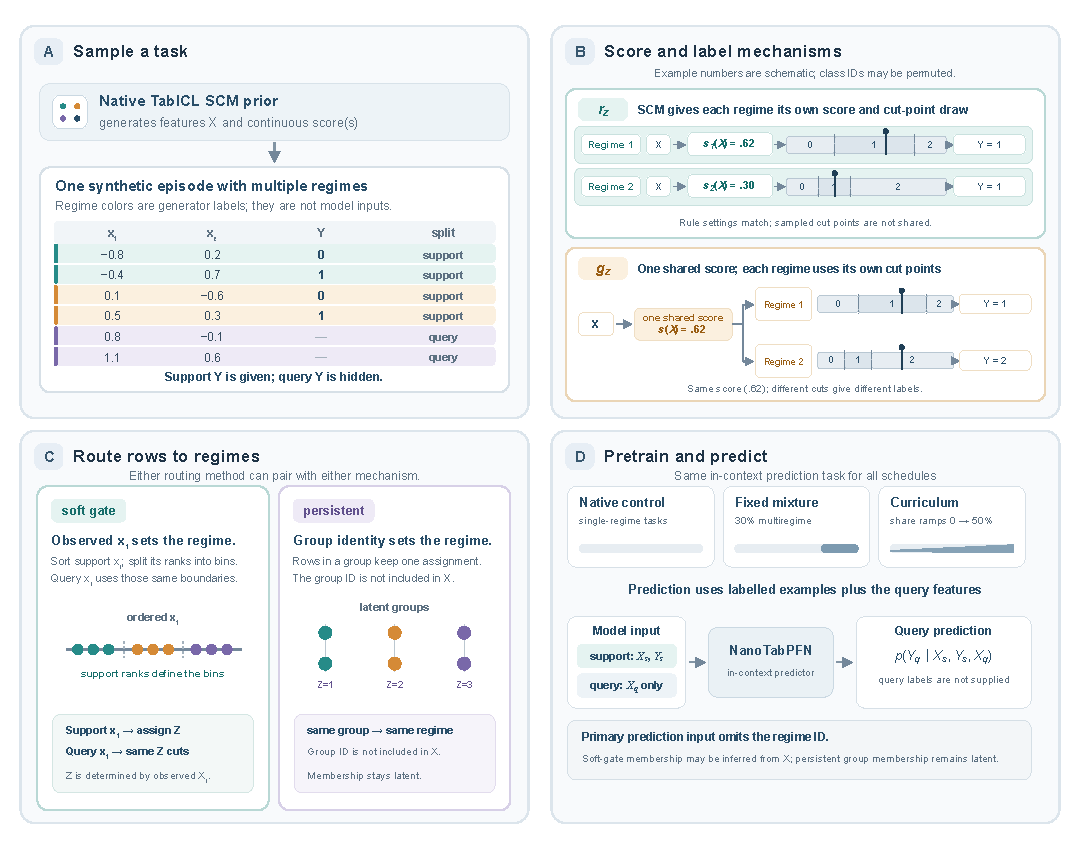
\includegraphics[width=.86\linewidth]{figure1_native_multiregime.pdf}
\caption{Native task construction. In $r_z$, regimes use separate SCM scores and independently drawn class cut points; in $g_z$, they share a score and use separate cut points. Soft-gate membership depends on observed $x_1$, while persistent membership is latent. The predictor sees support examples and query features, not regime IDs. The one-regime control, fixed 30\% mixture, and 0--50\% curriculum share the NanoTabPFN architecture.}
\label{fig:prior}
\end{figure}

\section{Experimental Setup}
We train matched native-control, fixed-mixture, and curriculum NanoTabPFN runs at three configurations (small/medium/large): 2 layers/64-dimensional embeddings/4 heads/256-wide MLP, 4/128/4/512, and 6/192/6/768. Thus size changes more than depth. Fixed mixing draws multiregime tasks in 30\% of batches; curriculum mixing ramps their share from 0 to 50\% over steps 1,000--5,000. All runs use initialization seed 2402, the same 10,000-step recipe and native one-regime task source; the two mixtures alternately use $r_z$ and $g_z$ task dumps (pre-generated synthetic episode files). We report final checkpoints, rather than selecting a favorable test checkpoint. Appendix~\ref{app:training} gives the recorded training recipe and its provenance limits.

The native control is essential to the estimand: a published PFN may use a different architecture, optimization path, and task prior. For each size, candidate and control checkpoints are evaluated on the same episode IDs, allowing per-episode subtraction before aggregation. The nine native runs share a nominal seed and recipe, but that is one training realization per condition. Differences across two-, four-, and six-layer configurations describe combined capacity changes because width and MLP size also increase. They should not be read as a depth-only ablation.

The standard-input native test bank varies $K=1$--4, binary or 3--5-class labels, binary imbalance, support size, feature count, mechanism, and routing family, including single-rule controls. Matched models see identical episodes. The headline multiregime multiclass subset contains 5,760 episodes in 720 factorial cells; its soft-gate and persistent halves have 2,880 episodes each. We also evaluate 36 selected BeyondArena tasks (27 binary, nine multiclass), with official folds and equal task weighting \citep{purucker2026beyondarena}. Appendix~\ref{app:beyond} documents those tasks and the independent evaluation protocol.

We define the headline subset before interpreting its results: $K\geq2$, a multiregime rule, and three to five classes. It contains both $r_z$ and $g_z$ mechanisms and both routing families, with eight episodes per factorial cell. The broader bank additionally contains binary, one-regime, and shared-rule controls; pooling all of them can obscure the behavior on the targeted tasks. BeyondArena evaluation is a separate transfer check on selected real datasets rather than a second sample from the synthetic prior; its evaluation partitions (IID, grouped, temporal) need not correspond to distinct latent label mechanisms, and its split summaries have especially few grouped and temporal tasks, which constrains their interpretation.

The factorial bank enforces a minimum of 32 labelled support rows per requested regime. Consequently, not every regime count occurs at every support size: since each regime needs at least 32 support rows, $K=4$ occurs only at support sizes 128, 256, and 512 (all but the smallest, 64), while $K=2$ occurs at every support size. We do not interpret a raw $K$ trend as an isolated effect of regime count. The $K=1$ branch checks behavior on native one-rule tasks, and shared-rule cells check the geometry of multiple assignments without changing the label rule by regime. The multiregime multiclass subset is the direct test of the training intervention, so it is reported separately from these controls. Matching episode identities across checkpoints removes evaluation-set composition as an explanation for their paired differences.

For each episode we report query cross-entropy (CE), accuracy gain over majority-class prediction (percentage points), and macro one-versus-rest AUC. Excess CE is model CE minus the CE of the empirical support-class-frequency predictor; smaller is better. Cross-entropy is a proper score, although a CE reduction by itself is not a calibration study \citep{gneiting2007scoring}. Published PFNs and conventional models use the same synthetic episodes in Table~\ref{tab:headline}. The baseline families include random forests, logistic regression, XGBoost, histogram gradient boosting, LightGBM, and CatBoost \citep{breiman2001forests,pedregosa2011sklearn,chen2016xgboost,ke2017lightgbm,prokhorenkova2018catboost}. TabPFN v2.6 is identified by its release card \citep{priorlabs2026tabpfn26}; Appendix~\ref{app:training} lists the configured published-model checkpoint names and the limits of their verification.

For native-model effects, we average within-cell paired candidate-minus-control differences and then give factorial cells equal weight. Negative CE differences and positive accuracy differences favor multiregime pretraining. The percentile intervals in Figure~\ref{fig:effects} resample evaluation episodes within cells; they quantify finite-bank variation conditional on frozen checkpoints and do not represent uncertainty across training seeds. Absolute Table~\ref{tab:headline} scores answer a complementary question about model ranking on the same subset. The baseline model families were not trained under the matched native recipe, so their gaps should not be interpreted as prior-only effects.

\paragraph{Additional analyses.} We run four further checks, reported in Section~5. First, we audit training-label balance for the native single-regime and pooled multiregime task dumps, in both the binary and multiclass setting, to test whether the multiregime advantage could instead reflect a change in class balance rather than regime structure. Second, we stratify the headline multiclass episodes by empirical support-label balance to check whether the routing effect is confined to a particular imbalance regime. Third, a frozen-checkpoint diagnostic appends a regime-tag column under three conditions -- hidden (no tag), shuffled (tag independently permuted within support and query), and true (realized membership, tags independently relabelled per episode) -- to measure what a supplied, aligned tag can add to prediction at matched input width (Appendix~\ref{app:diagnostic}). Fourth, for a real-data probe with an observed, non-synthetic group label, we merge three same-schema UCI Heart Disease sites into one 797-row dataset with an observed hospital label \citep{janosi1989heart}, evaluated under repeated stratified IID folds and a target-site adaptation protocol that keeps 20 stratified labelled target-site rows in support so the held-out site's category is genuinely observed rather than imputed (Appendix~\ref{app:heart}).

\section{Results}
\paragraph{Synthetic: matched headline comparison.} Table~\ref{tab:headline} uses the same 5,760 multiregime multiclass episodes for every model. The native single-regime model already improves over the support-frequency predictor: its excess CE is $-0.0838$ nats and accuracy gain is $6.30\pp$. Fixed and curriculum models reach $-0.0914$ and $-0.0926$ excess CE -- a 9.1\% and 10.5\% relative reduction from the native control, respectively; curriculum accuracy gain is $6.69\pp$, a 6.2\% relative increase over the native control's $6.30\pp$. Paired curriculum-minus-control CE is $-0.0088$ nats ($[-0.0094,-0.0082]$), and accuracy gain is $+0.38\pp$ ($[+0.34,+0.43]$). The fixed-mixture changes are $-0.0076$ nats and $+0.37\pp$. All published PFNs shown outperform the six-layer native variants on both headline metrics, and all six conventional classifiers trail them on this subset.

\begin{table}[t]
\caption{Matched standard-input synthetic multiregime multiclass comparison: 5,760 episodes, 720 cells, 3--5 classes. Direct query means; lower CE and higher accuracy are better. The three NanoTabPFN rows are six-layer final checkpoints.}
\label{tab:headline}\centering\small
\begin{tabular}{@{}lrr@{}}\toprule
Model & Query CE (nats) $\downarrow$ & Accuracy (\%) $\uparrow$ \\\midrule
Random forest & 1.2445 & 47.57\\
CatBoost & 1.2524 & 47.33\\
Logistic regression & 1.2832 & 44.54\\
XGBoost & 1.7099 & 45.44\\
Histogram gradient boosting & 1.7829 & 45.20\\
LightGBM & 2.5564 & 44.92\\\midrule
TabICL v1 & 1.1243 & 49.48\\
TabICL v1.1 & 1.1389 & 49.02\\
TabICL v2 & 1.1168 & 50.12\\
TabPFN v2.2 & 1.1040 & 50.55\\
TabPFN v2.6 & 1.1077 & 50.45\\
TabPFN v3 & 1.1031 & 50.59\\\midrule
NanoTabPFN, native single-regime & 1.1593 & 48.28\\
NanoTabPFN, fixed mixture & 1.1517 & 48.65\\
NanoTabPFN, curriculum & 1.1505 & 48.66\\\bottomrule
\end{tabular}
\end{table}

For reference, TabPFN v3 reaches 1.1031 CE and 50.59\% accuracy, compared with 1.1505 and 48.66\% for the curriculum model \citep{grinsztajn2026tabpfn3}. These are subset scores, distinct from full-bank scores in Appendix~\ref{app:synthetic}. The fixed and curriculum rows are close: on the headline subset their direct CE values differ by 0.0012 nats and their accuracies by 0.01 percentage points -- a much smaller separation than either model's gap to the native control. For instance, random forest and CatBoost have accuracies within roughly one point of the native control, yet their CE values are higher; accuracy and probability quality need not order methods identically.

\paragraph{Feature-dependent multiclass routing.} At six layers, soft-gate multiregime multiclass excess CE improves from $-0.1562$ for the native control to $-0.1730$ for curriculum training, a 10.8\% relative reduction. Across its 2,880 matched episodes, curriculum minus control CE is $-0.0168$ nats (95\% episode-bootstrap interval $[-0.0179,-0.0158]$), and accuracy gain changes by $+0.84\pp$ ($[+0.76,+0.91]$). The corresponding persistent-routing improvement is smaller: fixed mixing changes CE by $-0.0014$ nats ($[-0.0021,-0.0006]$) and accuracy by $+0.07\pp$ ($[0.00,0.13]$); curriculum changes them by $-0.0008$ nats and $-0.07\pp$.

\begin{figure}[t]
\centering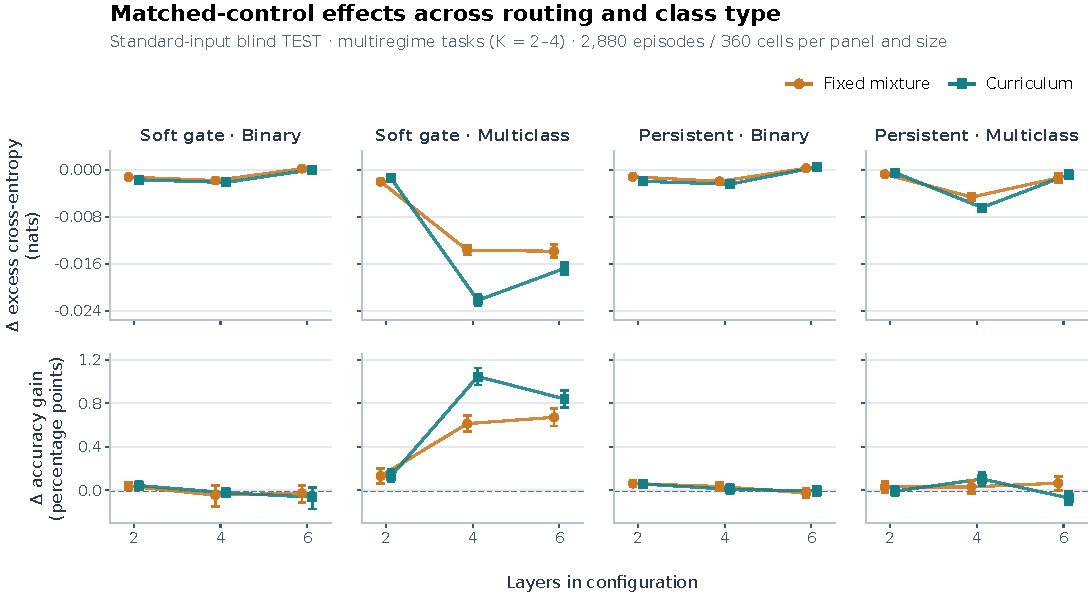
\includegraphics[width=.92\linewidth]{figure2_native_matched_effects.pdf}
\caption{Candidate-minus-same-size-native-control effects on the standard-input test bank, restricted to $K=2$--4. Each routing-by-class panel includes 2,880 episodes in 360 factorial cells per size. Points equally average cell means; whiskers are 95\% percentile intervals from 5,000 within-cell episode-bootstrap replicates. Negative CE and positive accuracy difference favor multiregime pretraining. Intervals omit pretraining-seed variation; model configurations vary in depth, width, and heads.}
\label{fig:effects}
\end{figure}

\paragraph{Rule mechanisms.} The improvement is not confined to one way of changing the label rule. Table~\ref{tab:mechanism} partitions the six-layer matched multiclass result into $r_z$ and $g_z$ episodes within each routing family. Under soft-gate routing, curriculum changes CE by $-0.0164$ nats for $r_z$ and $-0.0172$ for $g_z$, with accuracy gains of about $0.83$--$0.85\pp$; fixed mixing has smaller but similarly directed effects. In persistent tasks both mechanisms show CE differences below $0.002$ nats in magnitude, and curriculum accuracy differences are slightly negative. Thus the main routing contrast appears under both sampled rule constructions.

\begin{table}[t]
\centering\small
\caption{Matched six-layer candidate-minus-native effects by routing and rule mechanism on multiregime multiclass episodes. Each row has 1,440 episodes in 180 cells. Negative CE and positive accuracy differences (pp) favor the candidate.}
\label{tab:mechanism}
\begin{tabular}{@{}llrrrr@{}}\toprule
Routing & Rule & Fixed $\Delta$CE & Fixed $\Delta$Acc & Curr. $\Delta$CE & Curr. $\Delta$Acc\\\midrule
soft gate & $r_z$ & -0.0135 & +0.67 & -0.0164 & +0.83\\
soft gate & $g_z$ & -0.0142 & +0.67 & -0.0172 & +0.85\\
persistent & $r_z$ & -0.0018 & +0.01 & -0.0007 & -0.07\\
persistent & $g_z$ & -0.0009 & +0.12 & -0.0009 & -0.07\\
\bottomrule\end{tabular}
\end{table}


The routing contrast also appears at each requested multiclass count. In soft-gate tasks, curriculum minus native CE is $-0.0129$, $-0.0162$, and $-0.0213$ nats for three, four, and five classes, respectively, with 95\% episode-bootstrap intervals excluding zero in every case and positive accuracy differences in each slice. In persistent tasks, corresponding CE differences lie between $-0.0010$ and $-0.0004$ nats; only the three-class interval excludes zero, and the accuracy direction varies by class count. Each routing-by-class comparison uses 960 matched episodes in 120 cells. The class count changes the scale of CE and the label distribution, so we do not read these magnitudes as a monotone difficulty response.

\paragraph{Limits of the effect.} In multiregime binary tasks, the two- and four-layer native variants have positive excess CE, and six-layer models beat the support-frequency baseline by only about 0.003 nats. At six layers, curriculum changes binary CE by $+0.0003$ nats and accuracy by $-0.03\pp$ relative to its control. Four- and six-layer configurations show clearer multiclass changes than the two-layer configurations (Figure~\ref{fig:effects}). Across the entire standard-input test bank, six-layer fixed and curriculum CE is nearly identical (0.7802 and 0.7803).

\paragraph{Evaluation-balance sensitivity.} We stratify the same 5,760 episodes by the empirical support majority-class fraction, using tertile cutoffs separately for three, four, and five classes; cutoffs are chosen from labels before looking at model scores, and tied values stay in the lower bin. Table~\ref{tab:balance} averages paired effects within occupied factorial cells and then gives the three class counts equal weight. The six-layer curriculum soft-gate CE difference remains negative in low, middle, and high support-imbalance bins ($-0.0190$, $-0.0175$, and $-0.0132$ nats); fixed mixing is also favorable in each bin. In persistent tasks the effects are much smaller, and the highest-imbalance bin has a curriculum CE difference of $+0.0011$ nats. Appendix~\ref{app:synthetic} reports all class-count slices and their episode and cell counts.

\begin{table}[t]
\centering\footnotesize
\caption{Evaluation-balance sensitivity on the existing standard-input bank. Six-layer candidate minus native-control paired effects; lower CE and higher accuracy differences (pp) favor the candidate. Bins are defined by support majority fraction within each class count, without using outcomes; pooled rows give class counts equal weight. Descriptive fixed-checkpoint contrasts, not a control for training-label balance.}\label{tab:balance}
\begin{tabular}{@{}llrrrrrr@{}}\toprule
Routing & Maj. bin & $n$ & Cells & Fixed $\Delta$CE & Fixed $\Delta$Acc & Curr. $\Delta$CE & Curr. $\Delta$Acc\\\midrule
soft gate & low & 989 & 340 & -0.0154 & +0.72 & -0.0190 & +1.09\\
soft gate & middle & 970 & 348 & -0.0144 & +0.65 & -0.0175 & +0.81\\
soft gate & high & 921 & 332 & -0.0102 & +0.42 & -0.0132 & +0.51\\
persistent & low & 981 & 335 & -0.0029 & +0.19 & -0.0022 & +0.04\\
persistent & middle & 985 & 348 & -0.0020 & +0.13 & -0.0015 & -0.11\\
persistent & high & 914 & 334 & +0.0000 & -0.08 & +0.0011 & -0.12\\
\bottomrule\end{tabular}
\end{table}


\paragraph{Training-label balance.} In a binary training-dump diagnostic, the mean majority-class fraction is 0.766 for the native single-regime dump and 0.66 for pooled multiregime dumps (Appendix~\ref{app:prior}). The corresponding multiclass comparison across three, four, and five requested classes shows the same pattern: multiregime dumps are more balanced than the native dump at every class count (Appendix~\ref{app:prior}).

\paragraph{Supplied regime-tag diagnostic.} Within each mechanism-by-routing stratum (1,440 matched multiclass episodes, 180 cells), true-minus-shuffled CE ranges from $-0.174$ to $-0.057$ nats for persistent $r_z$ and $-0.179$ to $-0.058$ for persistent $g_z$, with accuracy changes of $+4.48$ to $+11.32\pp$ and $+4.62$ to $+11.69\pp$. For soft-gate $r_z$ and $g_z$, CE changes range from $-0.062$ to $-0.034$ nats, with accuracy changes of $+1.99$ to $+3.64\pp$ and $+2.16$ to $+3.67\pp$. Shuffled-minus-hidden is near zero for persistent tasks ($-0.0023$ to $+0.0011$ nats) but raises CE by $0.0022$--$0.0057$ on soft-gate tasks -- an effect of appending a feature, not of its alignment. Appendix~\ref{app:diagnostic} reports the full size-by-model contrasts, their paired intervals, and why these frozen checkpoints cannot support a per-regime recovery analysis.

\paragraph{Real data: BeyondArena transfer.} On 36 selected BeyondArena tasks, six-layer curriculum-minus-native-control excess CE is approximately $+0.0036$ nats and accuracy gain $-0.10\pp$ (descriptive differences from rounded task-level values); the fixed mixture is similarly close to the control. Published TabICLv2 and TabPFN v3 outperform the native models on the reported aggregates (Appendix~\ref{app:beyond}). The rounded task-level CE comparison is mixed in sign: curriculum is lower on 16 tasks, tied on two at printed precision, and higher on 18. By split, CE differences are $+0.0021$ (32 IID tasks), $+0.0187$ (three grouped), and $+0.0070$ (one temporal).

\paragraph{Merged heart-site case study.} In the merged heart-site case study (Appendix~\ref{app:heart}), an observed hospital label has little effect under repeated stratified IID folds: excess CE changes by at most 0.0045 nats across the 20 evaluated models, with no consistent direction. In the target-site adaptation protocol, the aligned-minus-shuffled site-tag contrast in excess CE ranges from $-0.0127$ to $+0.0042$ across the same 20 models, with 16 of 20 negative; the largest gains are for TabICL v1, random forest, and the medium native configurations. Multiregime pretraining shows no consistent additional advantage over the native single-regime control at any one size.

\FloatBarrier
\section{Discussion and Limitations}
The designed prior produces a measurable but modest synthetic advantage concentrated in feature-dependent multiclass tasks. Soft-gate routing makes regime information available in $x_1$; persistent assignments are not directly supplied. The weak binary results and small persistent-routing effects prevent a broad claim about multiregime classification; as Section~2 notes, this improvement also does not establish reconstruction or identifiability of latent memberships (Limitations). The tag intervention in Appendix~\ref{app:diagnostic} shows that aligned membership can improve prediction, especially for persistent tasks, but it supplies privileged information to the predictor.

The matched synthetic design answers a narrow question: for these checkpoints and this generated distribution, replacing some native one-regime tasks with multiregime tasks helps on selected multiclass evaluations. It does not show that the model uses an explicit routing algorithm or recovers the generator's row assignments. Near-zero persistent effects indicate little predictive benefit when query membership is unobserved, not that regimes are absent. The supplied-tag diagnostic changes evaluation-time information and tests a different counterfactual.

The training-label balance audit shows multiregime dumps are more balanced in the multiclass setting, so gains could reflect class distribution as well as regime structure; it does not quantify their contributions. Fixed and curriculum mixtures also differ in total multiregime exposure (Section~3), so the comparison supports no specific scheduling explanation. Published PFNs remain stronger on both headline metrics. The soft-gate effect appears in CE and accuracy at six layers, while persistent effects are small and their accuracy direction varies by schedule. This is consistent with useful information in observed $x_1$, but predictive scores do not reveal whether the model recovered memberships. Evaluation-balance slices show the soft-gate advantage across imbalance bins, but this descriptive test-bank analysis leaves the training-label confound intact. A decisive comparison would equalize training class balance while varying regime structure and use independent seeds; the current post-hoc slices are exploratory.

Neutral transfer on BeyondArena therefore does not show that real data lack heterogeneity. The same caution applies to accuracy and AUC in that comparison, because different tasks, target types, and split designs contribute to their aggregates. A grouped fold tests prediction for a held-out group; it does not tell us whether the group index is sufficient for the label rule or whether the synthetic prior's feature-dependent gate is a good approximation. We interpret the real-data results as evidence about these evaluated checkpoints on this selected suite, rather than as validation of the generator's mechanism.

Equal task weighting prevents larger datasets from dominating, but 36 selected tasks do not represent every tabular setting; Appendix~\ref{app:beyond} retains task-level scores. The three grouped tasks split many small groups, averaging as few as 2--12 rows per group, which limits split-specific conclusions. The heart-site intervention shows that an observed group label can affect target-site prediction, but does not recreate an unobserved $r_z$ or $g_z$ process.

The synthetic and real-data evaluations therefore stress different capabilities. In the synthetic soft gate, a designated observed coordinate helps determine membership under the generator. In a real dataset, candidate grouping cues can be distributed among features, absent for new groups, or irrelevant to the conditional label rule. The merged heart data offer one concrete observed-site probe, but the model is scored on disease prediction, not on reconstructing a hidden site or verifying distinct causal mechanisms. Its repeated target-site draws reuse most query rows, so they do not provide 15 independent dataset-level tests. A real-data gain would need to be established on more tasks with documented environment labels and matched training controls. The neutral results here put a bound on what these particular pretraining mixtures achieved, while leaving open whether another prior or architecture would transfer better.

\paragraph{Limitations.} All main-model comparisons use one pretraining seed; paired episode-bootstrap intervals quantify test-bank variation for frozen checkpoints, not variation from retraining, model weights, or training streams. Thousands of matched episodes make the fixed-checkpoint CE differences estimable on this bank, but the intervals also do not account for selecting this prior, subset, or diagnostic after looking at earlier experiments. We report CE and accuracy together because a change in predictive probabilities can matter even when the winning class changes rarely; conversely, a small accuracy gain does not show that a model's probabilities are calibrated. The weak binary and persistent results are part of the same evidence, not exceptions to be discarded in favor of the soft-gate multiclass slice. Predictive improvement anywhere in this study, including under the supplied regime tag, does not establish reconstruction or identifiability of latent memberships. More seeds, broader grouped and temporal coverage, and prior designs closer to real mechanisms are needed before a general transfer claim.

\section{Conclusion}
Multiregime-mixture pretraining improves compact PFN prediction on synthetic multiclass tasks, most clearly when feature values provide routing cues. For the six-layer model on these feature-dependent tasks, curriculum pretraining improves excess cross-entropy by 10.8\% relative to the native prior; across all multiregime multiclass tasks, accuracy gain over majority prediction rises from 6.30 to 6.69 percentage points. Fixed-mixture pretraining also improves the pooled benchmark, so the gains are not unique to the curriculum schedule. The selected BeyondArena and merged heart-site evaluations show no consistent transfer advantage. These findings show that PFNs can benefit from priors that include coexisting label rules and motivate further work on multiregime tabular learning.

\subsubsection*{AI use statement}
Generative AI assisted with code, experiment execution, analysis, figures, manuscript drafting and editing, tables, and PDF checks, including the balance-slice analysis reported here. The authors report human checks of the manuscript, literature review, tables, experiments, analysis, data preprocessing, code, and figures, and retain responsibility for the final claims and submission. The literature review, data preprocessing, experiment design, and formulation of research ideas were not AI-assisted.

\subsubsection*{Reproducibility statement}
The prior and controls are specified in Sections 3--4 and Appendices~\ref{app:prior}--\ref{app:training}; headline synthetic and real-data figures are reported in Section~5, with full task-level tables in Appendices~\ref{app:synthetic}, \ref{app:beyond}, and \ref{app:heart}. The September native training used the TabICL SCM from \texttt{tabicl} 2.1.1 and TFM-Playground 0.0.1; Appendix~\ref{app:training} records package and checkpoint identifiers available locally. The balance analysis joins report episode IDs to the saved standard-input test bank without model inference. The 36-task container and official-fold archive, including an immutable BeyondArena revision, is described in Appendix~\ref{app:beyond}; the BeyondArena revision hash is provided in the supplementary materials. No anonymous public release is available at drafting time. The saved records omit the historical source commit, checkpoint content hashes, and the 36-task job's cached dataset revision; the pinned archive matches available task records but does not establish the job's exact cache identity.

\bibliographystyle{iclr2027_conference}
\bibliography{references}
\clearpage\appendix
\section*{Appendix}

\section{Native Prior and Implementation Validation}\label{app:prior}
The native generator draws TabICL SCM hyperparameters using its fixed and sampled defaults, obtains feature columns and one or more continuous score columns, and applies native \texttt{Reg2Cls} score-to-class conversion. A sampled score-to-label rule draws class cut points and may permute class IDs. For $r_z$, each of $K$ score columns receives an independent cut-point draw under the same cut-point settings; for $g_z$, one score is reused with $K$ independent conversions. The rule active for row $i$ is selected by $z_i$. With $K=1$, the implementation follows the native TabICL prior path; the documented validation checked bit-identical output against \texttt{tabicl.prior.PriorDataset} for both mechanism settings. The selected labels pass TabICL's split sanity check, and episodes with non-finite feature values are redrawn. The recorded dump invocation is in \path{scripts/slurm/dump_multiregime_v4_native.sbatch}; its historical source commit was not logged.

The primary evaluation uses a factorial bank with $K=1$--4, binary and 3--5-class outcomes, 0.1/0.3/0.5 controlled binary class-ratio cells, varied support sizes and feature counts, the two rule mechanisms, and soft-gate or persistent assignment. Soft-gate cut points are based on ranks of observed $x_1$ in the support set. Persistent assignment remains a stable latent group label and is not supplied in the standard input. Multiclass evaluation cells require each requested class to appear. Native pretraining itself produces imbalanced classes. In the documented binary training dumps, the native single-regime tasks have mean majority-class fraction 0.766, with 45\% of tasks at or above 0.8; pooling multiregime rules gives 0.66 and 15\%, respectively. Per-regime label balance has the native spread, so pooling independent rules moves binary tasks toward balance. Across all 100,000 episodes in each local native single-regime, $r_z$, and $g_z$ training dump, for three, four, and five requested classes respectively, mean support-majority fractions are 0.638, 0.551, and 0.491 for the native dump; 0.517, 0.432, and 0.376 for $r_z$; and 0.515, 0.431, and 0.374 for $g_z$ (12,461/12,444/12,481 episodes per class count, giving episodes equal weight within each requested class count; these describe the source dumps rather than the realized schedule-weighted training stream). Multiregime tasks are therefore more balanced on average in both the binary and multiclass settings; Section~5 (Training-label balance) reports the pooled summary. The earlier non-native generator calibrated classes to fixed balanced vectors and is excluded from this study.

\section{Architectures and Training Reproducibility}\label{app:training}
\begin{table}[h]\centering\small
\caption{Recorded NanoTabPFN configurations. These are size configurations, not a depth-only ablation.}\label{tab:arch}
\begin{tabular}{@{}lrrrr@{}}\toprule Size & Layers & Embedding & Heads & MLP hidden\\\midrule
Small & 2 & 64 & 4 & 256\\ Medium & 4 & 128 & 4 & 512\\ Large & 6 & 192 & 6 & 768\\\bottomrule\end{tabular}\end{table}
Each condition uses seed 2402, 10,000 steps, batch size four with 32 accumulated gradients, learning rate $10^{-4}$, minimum $10^{-6}$, 2,000-step warmup, weight decay 0.01, and gradient clipping at 1.0. Training tasks have 1,024 rows, 2--12 features, 2--5 classes, and a sampled training fraction between 0.1 and 0.9. The ordinary branch uses the one-regime dump; the multiregime branch alternates $r_z$ and $g_z$ dumps. Fixed mixing uses 30\% multiregime batches. The curriculum reaches a 50\% share over steps 1,000--5,000. Validation is recorded every 500 steps on the native bank and a separate 16-batch stream; the results here use step-10,000 final checkpoints. The configuration is recorded in \texttt{scripts/slurm/pretrain\_multiregime\_v4\_native.sbatch}; the nine saved \texttt{config.json} files under \path{artifacts/cluster_sync/tfm_runs/native/} confirm the size-specific values in Table~\ref{tab:arch}. Their standard-input final-test reports are under \path{artifacts/cluster_sync/tfm_eval/native_regime_split/blind/}.

The authors confirmed that the project \texttt{uv.lock} was the training lock for these September native runs. It records TabICL 2.1.1, TabPFN 8.5.0, and Data Foundry 0.0.5; NanoTabPFN is repository source rather than a separately versioned package. The nine native checkpoint identifiers are \texttt{original}, \texttt{rg\_z-fixed}, and \texttt{rg\_z-curriculum}, each at small, medium, and large size, seed 2402, and final step 10,000. The published-model evaluation script names TabICL checkpoint files \path{tabicl-classifier-v1-20250208.ckpt}, \path{tabicl-classifier-v1.1-20250506.ckpt}, and \path{tabicl-classifier-v2-20260212.ckpt}; the Slurm defaults identify TabPFN files \path{tabpfn-v2.2.ckpt}, \path{tabpfn-v2.6-classifier-v2.6_default.ckpt}, and \path{tabpfn-v3-classifier-v3_default.ckpt}. These names identify configured files, not verified content hashes. The synced run records contain configuration and evaluation reports but no native checkpoint binaries or historical source commit. Thus checkpoint content, published file identities, and shared initialization from saved states could not be independently verified from these records.

\section{Additional Synthetic Results}\label{app:synthetic}
\begin{table}[h]\centering\small
\caption{Final standard-input test-bank scores pooled across task conditions. Accuracy is a fraction. This full-bank comparison has a different composition from Table~\ref{tab:headline}.}\label{tab:fullbank}
\begin{tabular}{@{}llrrr@{}}\toprule Size & Prior & CE & Excess CE & Accuracy\\\midrule
Small & Native & .8164 & $-.0192$ & .6178\\ & Fixed & .8157 & $-.0199$ & .6182\\ & Curriculum & .8161 & $-.0195$ & .6179\\
Medium & Native & .8095 & $-.0261$ & .6304\\ & Fixed & .8053 & $-.0303$ & .6312\\ & Curriculum & .8036 & $-.0320$ & .6317\\
Large & Native & .7811 & $-.0545$ & .6385\\ & Fixed & .7802 & $-.0554$ & .6393\\ & Curriculum & .7803 & $-.0553$ & .6389\\\bottomrule\end{tabular}\end{table}
Table~\ref{tab:fullbank} includes one-regime, shared-rule, binary, and multiclass cells and therefore dilutes the multiregime multiclass headline effect. The standard-input bank is primary. Across multiregime binary cells, the two smaller configurations have positive excess CE, and large configurations have only a small negative excess CE. The large soft-gate multiclass gain and small persistent gain are quantified in Section 5 and Figure~\ref{fig:effects}. Per-cell trajectories on the standard-input and legacy duplicate-X1 banks appear in Figure~\ref{fig:cells}, and training/validation curves for all three sizes appear in Figure~\ref{fig:history}. The paired analysis uses 5,000 percentile-bootstrap replicates resampled within each factorial cell (seed 20260924); intervals are unadjusted descriptive intervals across evaluation episodes. Fixed mixing and curriculum differ both in temporal schedule and multiregime exposure, preventing a pure scheduling attribution.

Tables~\ref{tab:balance-soft_gate} and~\ref{tab:balance-persistent} expand the main-text support-balance analysis by requested class count. The support-majority tertile cutoffs are 0.4473 and 0.5313 for three classes, 0.3672 and 0.4375 for four classes, and 0.3164 and 0.3789 for five classes. Discrete support-label counts create ties, so bin episode counts are unequal. Across all nine soft-gate class-by-balance slices the six-layer fixed and curriculum CE differences are negative; persistent differences are smaller and are not uniformly favorable. These are scores for the original bank under its observed label frequencies. No evaluation episodes were regenerated and no model was retrained for this diagnostic.

The companion machine-readable balance report records SHA-256 hashes of the local test bank and verified training lock. Its alignment check compares every report episode's metadata with the local bank and confirms all binary support and query class fractions. The saved evaluation reports do not retain multiclass labels, so complete label-level equivalence to the unavailable cluster-side HDF5 file cannot be independently checked from these reports alone.

\begin{table}[ht]
\centering\footnotesize
\caption{Detailed soft gate evaluation-balance slices. Candidate minus same-size native control; accuracy differences are percentage points. Cell means are weighted equally within each class-count slice. Support-majority cutoffs are shared across routing families within class count.}\label{tab:balance-soft_gate}
\begin{tabular}{@{}lllrrrrrr@{}}\toprule
Classes & Routing & Maj. bin & $n$ & Cells & Fixed $\Delta$CE & Fixed $\Delta$Acc & Curr. $\Delta$CE & Curr. $\Delta$Acc\\\midrule
3 & soft gate & low & 324 & 113 & -0.0112 & +0.90 & -0.0152 & +1.08\\
4 & soft gate & low & 348 & 115 & -0.0176 & +0.70 & -0.0197 & +1.08\\
5 & soft gate & low & 317 & 112 & -0.0174 & +0.56 & -0.0221 & +1.10\\
3 & soft gate & middle & 337 & 117 & -0.0105 & +0.39 & -0.0139 & +0.69\\
4 & soft gate & middle & 302 & 115 & -0.0134 & +0.64 & -0.0154 & +0.62\\
5 & soft gate & middle & 331 & 116 & -0.0192 & +0.93 & -0.0233 & +1.12\\
3 & soft gate & high & 299 & 109 & -0.0051 & +0.38 & -0.0094 & +0.51\\
4 & soft gate & high & 310 & 110 & -0.0127 & +0.48 & -0.0117 & +0.44\\
5 & soft gate & high & 312 & 113 & -0.0129 & +0.39 & -0.0186 & +0.59\\
\bottomrule\end{tabular}
\end{table}

\begin{table}[ht]
\centering\footnotesize
\caption{Detailed persistent evaluation-balance slices. Candidate minus same-size native control; accuracy differences are percentage points. Cell means are weighted equally within each class-count slice. Support-majority cutoffs are shared across routing families within class count.}\label{tab:balance-persistent}
\begin{tabular}{@{}lllrrrrrr@{}}\toprule
Classes & Routing & Maj. bin & $n$ & Cells & Fixed $\Delta$CE & Fixed $\Delta$Acc & Curr. $\Delta$CE & Curr. $\Delta$Acc\\\midrule
3 & persistent & low & 318 & 113 & -0.0006 & +0.09 & -0.0021 & +0.08\\
4 & persistent & low & 331 & 110 & -0.0036 & +0.50 & -0.0022 & +0.21\\
5 & persistent & low & 332 & 112 & -0.0046 & -0.01 & -0.0023 & -0.18\\
3 & persistent & middle & 335 & 115 & -0.0013 & +0.11 & -0.0013 & -0.12\\
4 & persistent & middle & 335 & 115 & -0.0035 & +0.20 & -0.0026 & +0.01\\
5 & persistent & middle & 315 & 118 & -0.0012 & +0.10 & -0.0007 & -0.22\\
3 & persistent & high & 307 & 110 & +0.0001 & -0.05 & +0.0007 & -0.06\\
4 & persistent & high & 294 & 112 & +0.0018 & -0.17 & +0.0032 & -0.12\\
5 & persistent & high & 313 & 112 & -0.0018 & -0.01 & -0.0005 & -0.18\\
\bottomrule\end{tabular}
\end{table}


\begin{figure}[h]\centering\includegraphics[width=.92\linewidth]{native_large_excess_ce_cells_test.png}
\caption{Six-layer native-prior test excess CE by task condition and checkpoint. Solid curves use standard input; dashed curves use duplicate-X1 input (a legacy diagnostic feature, not a true regime ID). Final-checkpoint diamonds are descriptive; matched final comparisons support the headline result.}\label{fig:cells}\end{figure}
\begin{figure}[h]\centering\includegraphics[width=.9\linewidth]{native_history.png}
\caption{Validation and training trajectories for the three size configurations. Rows show native-bank validation CE, the fixed validation stream, training query CE, and multiregime training-batch share. These diagnostics are distinct from held-out final test comparisons.}\label{fig:history}\end{figure}

\FloatBarrier
\section{Supplied Regime-Tag Diagnostic}\label{app:diagnostic}
\paragraph{Aligned membership as privileged input.} A frozen-checkpoint diagnostic evaluates the same 5,760 multiregime multiclass episodes for original, fixed, and curriculum models at all three sizes. The \emph{hidden} condition uses the ordinary features, \emph{shuffled} appends a regime-tag column independently shuffled within support and query, and \emph{true} appends the realized membership. Tag IDs are independently relabelled per episode. True minus shuffled compares aligned membership with a same-width corrupted tag; shuffled minus hidden detects effects from merely appending a feature. The test bank is shared with other analyses, so this is an exploratory diagnostic, not a new untouched test. Section~5 reports the headline true-minus-shuffled and shuffled-minus-hidden ranges; Tables~\ref{tab:tagcontrasts}--\ref{tab:tagaccuracy} below give the full size-by-model contrasts and their paired intervals. Figures~\ref{fig:tag-input-pooled}--\ref{fig:tag-input-gz} visualize these input-condition contrasts pooled across and split by SCM mechanism. The 5,000 cell-stratified bootstrap replicates describe finite-bank, not training-seed, uncertainty, and show predictive benefit from a \emph{supplied} aligned tag, not recovery of an unobserved regime.

\begingroup\footnotesize\setlength{\tabcolsep}{4pt}\setlength\LTleft{0pt}\setlength\LTright{0pt}
\begin{longtable}{@{}lllp{4.4cm}r@{}}
\caption{Within-checkpoint cross-entropy contrasts (nats) on multiregime multiclass episodes. True minus shuffled isolates aligned membership at matched input width; shuffled minus hidden captures an appended corrupted tag. Brackets are 95\% within-cell episode-bootstrap intervals (5,000 replicates), not training-seed intervals. Each mechanism-by-routing stratum has 1,440 episodes in 180 cells. O/F/C denote original/fixed/curriculum and S/M/L denote size.}\label{tab:tagcontrasts}\\
\toprule Mechanism & Routing & Model/size & True$-$shuffled [95\% interval] & Shuffled$-$hidden\\\midrule\endfirsthead
\multicolumn{5}{l}{\emph{Continued from previous page}}\\\toprule Mechanism & Routing & Model/size & True$-$shuffled [95\% interval] & Shuffled$-$hidden\\\midrule\endhead
\bottomrule\endfoot
$r_z$ & persistent & O/S & -0.057 [-0.061, -0.054] & +0.0008\\
$r_z$ & persistent & F/S & -0.059 [-0.063, -0.055] & +0.0007\\
$r_z$ & persistent & C/S & -0.058 [-0.061, -0.054] & +0.0008\\
$r_z$ & persistent & O/M & -0.150 [-0.156, -0.144] & -0.0023\\
$r_z$ & persistent & F/M & -0.158 [-0.164, -0.152] & -0.0012\\
$r_z$ & persistent & C/M & -0.164 [-0.170, -0.157] & -0.0018\\
$r_z$ & persistent & O/L & -0.162 [-0.169, -0.156] & -0.0005\\
$r_z$ & persistent & F/L & -0.172 [-0.178, -0.165] & -0.0004\\
$r_z$ & persistent & C/L & -0.174 [-0.180, -0.167] & -0.0005\\
\midrule
$r_z$ & soft gate & O/S & -0.035 [-0.037, -0.032] & +0.0048\\
$r_z$ & soft gate & F/S & -0.035 [-0.037, -0.032] & +0.0046\\
$r_z$ & soft gate & C/S & -0.034 [-0.037, -0.032] & +0.0048\\
$r_z$ & soft gate & O/M & -0.062 [-0.065, -0.058] & +0.0057\\
$r_z$ & soft gate & F/M & -0.057 [-0.060, -0.053] & +0.0046\\
$r_z$ & soft gate & C/M & -0.054 [-0.057, -0.050] & +0.0037\\
$r_z$ & soft gate & O/L & -0.042 [-0.046, -0.039] & +0.0044\\
$r_z$ & soft gate & F/L & -0.038 [-0.042, -0.035] & +0.0025\\
$r_z$ & soft gate & C/L & -0.037 [-0.040, -0.033] & +0.0024\\
\midrule
$g_z$ & persistent & O/S & -0.058 [-0.061, -0.055] & +0.0009\\
$g_z$ & persistent & F/S & -0.059 [-0.062, -0.056] & +0.0010\\
$g_z$ & persistent & C/S & -0.058 [-0.061, -0.055] & +0.0011\\
$g_z$ & persistent & O/M & -0.155 [-0.161, -0.149] & -0.0002\\
$g_z$ & persistent & F/M & -0.161 [-0.167, -0.155] & -0.0003\\
$g_z$ & persistent & C/M & -0.167 [-0.173, -0.161] & -0.0008\\
$g_z$ & persistent & O/L & -0.167 [-0.173, -0.160] & -0.0002\\
$g_z$ & persistent & F/L & -0.177 [-0.183, -0.170] & -0.0001\\
$g_z$ & persistent & C/L & -0.179 [-0.185, -0.172] & -0.0001\\
\midrule
$g_z$ & soft gate & O/S & -0.035 [-0.038, -0.032] & +0.0049\\
$g_z$ & soft gate & F/S & -0.035 [-0.037, -0.032] & +0.0047\\
$g_z$ & soft gate & C/S & -0.034 [-0.037, -0.031] & +0.0048\\
$g_z$ & soft gate & O/M & -0.062 [-0.066, -0.058] & +0.0045\\
$g_z$ & soft gate & F/M & -0.058 [-0.062, -0.054] & +0.0039\\
$g_z$ & soft gate & C/M & -0.056 [-0.059, -0.052] & +0.0033\\
$g_z$ & soft gate & O/L & -0.044 [-0.048, -0.040] & +0.0041\\
$g_z$ & soft gate & F/L & -0.040 [-0.044, -0.037] & +0.0026\\
$g_z$ & soft gate & C/L & -0.038 [-0.042, -0.035] & +0.0022\\
\end{longtable}\endgroup
\begingroup\footnotesize\setlength{\tabcolsep}{4pt}\setlength\LTleft{0pt}\setlength\LTright{0pt}
\begin{longtable}{@{}lllp{4.4cm}r@{}}
\caption{Within-checkpoint accuracy contrasts (percentage points) on multiregime multiclass episodes. True minus shuffled isolates aligned membership at matched input width; shuffled minus hidden captures an appended corrupted tag. Brackets are 95\% within-cell episode-bootstrap intervals (5,000 replicates), not training-seed intervals. Each mechanism-by-routing stratum has 1,440 episodes in 180 cells. O/F/C denote original/fixed/curriculum and S/M/L denote size.}\label{tab:tagaccuracy}\\
\toprule Mechanism & Routing & Model/size & True$-$shuffled [95\% interval] & Shuffled$-$hidden\\\midrule\endfirsthead
\multicolumn{5}{l}{\emph{Continued from previous page}}\\\toprule Mechanism & Routing & Model/size & True$-$shuffled [95\% interval] & Shuffled$-$hidden\\\midrule\endhead
\bottomrule\endfoot
$r_z$ & persistent & O/S & +4.52 [+4.18, +4.86] & -0.07\\
$r_z$ & persistent & F/S & +4.58 [+4.24, +4.93] & -0.03\\
$r_z$ & persistent & C/S & +4.48 [+4.14, +4.82] & -0.08\\
$r_z$ & persistent & O/M & +10.15 [+9.72, +10.57] & -0.05\\
$r_z$ & persistent & F/M & +10.56 [+10.12, +10.99] & -0.07\\
$r_z$ & persistent & C/M & +10.89 [+10.44, +11.34] & +0.00\\
$r_z$ & persistent & O/L & +10.85 [+10.41, +11.29] & -0.08\\
$r_z$ & persistent & F/L & +11.25 [+10.80, +11.69] & +0.01\\
$r_z$ & persistent & C/L & +11.32 [+10.87, +11.77] & -0.05\\
\midrule
$r_z$ & soft gate & O/S & +2.89 [+2.63, +3.17] & -0.39\\
$r_z$ & soft gate & F/S & +2.69 [+2.41, +2.97] & -0.35\\
$r_z$ & soft gate & C/S & +2.68 [+2.42, +2.97] & -0.36\\
$r_z$ & soft gate & O/M & +3.64 [+3.40, +3.89] & -0.36\\
$r_z$ & soft gate & F/M & +3.18 [+2.94, +3.43] & -0.26\\
$r_z$ & soft gate & C/M & +3.01 [+2.76, +3.26] & -0.23\\
$r_z$ & soft gate & O/L & +2.50 [+2.25, +2.75] & -0.22\\
$r_z$ & soft gate & F/L & +2.18 [+1.95, +2.42] & -0.14\\
$r_z$ & soft gate & C/L & +1.99 [+1.76, +2.24] & -0.14\\
\midrule
$g_z$ & persistent & O/S & +4.62 [+4.29, +4.96] & -0.12\\
$g_z$ & persistent & F/S & +4.72 [+4.39, +5.07] & -0.10\\
$g_z$ & persistent & C/S & +4.67 [+4.33, +5.02] & -0.11\\
$g_z$ & persistent & O/M & +10.67 [+10.23, +11.12] & -0.08\\
$g_z$ & persistent & F/M & +10.96 [+10.51, +11.41] & +0.00\\
$g_z$ & persistent & C/M & +11.26 [+10.81, +11.73] & -0.06\\
$g_z$ & persistent & O/L & +11.20 [+10.71, +11.68] & -0.07\\
$g_z$ & persistent & F/L & +11.59 [+11.11, +12.07] & -0.09\\
$g_z$ & persistent & C/L & +11.69 [+11.22, +12.18] & -0.01\\
\midrule
$g_z$ & soft gate & O/S & +2.69 [+2.42, +2.98] & -0.27\\
$g_z$ & soft gate & F/S & +2.62 [+2.35, +2.89] & -0.28\\
$g_z$ & soft gate & C/S & +2.57 [+2.31, +2.84] & -0.32\\
$g_z$ & soft gate & O/M & +3.67 [+3.39, +3.95] & -0.27\\
$g_z$ & soft gate & F/M & +3.41 [+3.12, +3.69] & -0.30\\
$g_z$ & soft gate & C/M & +3.01 [+2.74, +3.29] & -0.20\\
$g_z$ & soft gate & O/L & +2.71 [+2.45, +2.98] & -0.31\\
$g_z$ & soft gate & F/L & +2.35 [+2.08, +2.63] & -0.23\\
$g_z$ & soft gate & C/L & +2.16 [+1.91, +2.42] & -0.19\\
\end{longtable}\endgroup


\begin{figure}[h]\centering\includegraphics[width=.88\linewidth]{regime_information_prediction_comparison_r_z.png}
\caption{Frozen native-model differences from the original control for $r_z$ episodes under hidden, shuffled, and true membership inputs. Rows separate routing families and metrics; columns separate model sizes. Whiskers show paired within-cell episode-bootstrap intervals. The reports do not identify separately trained true-tag checkpoints.}\label{fig:rz}\end{figure}
\begin{figure}[h]\centering\includegraphics[width=.88\linewidth]{regime_information_prediction_comparison_g_z.png}
\caption{As in Figure~\ref{fig:rz}, for $g_z$ episodes. The within-model true-minus-shuffled contrast is the relevant supplied-information comparison.}\label{fig:gz}\end{figure}

\begin{figure}[h]\centering\includegraphics[width=\linewidth]{regime_information_input_effects.png}
\caption{Paired input-condition contrasts pooled across the $r_z$ and $g_z$ mechanisms. Columns show model size; rows show cross-entropy and accuracy changes for shuffled versus hidden and true versus shuffled inputs under persistent and soft-gate routing. Each routing family includes 2,880 matched episodes. Dots are paired mean differences; bars are 95\% cell-stratified episode-bootstrap intervals over this fixed bank, not training-seed uncertainty. Negative cross-entropy and positive accuracy changes favor the first-named condition.}\label{fig:tag-input-pooled}\end{figure}
\begin{figure}[h]\centering\includegraphics[width=\linewidth]{regime_information_conditions_r_z.png}
\caption{Within-model paired input-condition contrasts for $r_z$ episodes. Panels show cross-entropy and accuracy changes for shuffled versus hidden and true versus shuffled inputs across sizes and routing families. Each routing family includes 1,440 matched episodes. Dots are paired means and bars are 95\% cell-stratified episode-bootstrap intervals over this fixed bank, not training-seed uncertainty. Negative cross-entropy and positive accuracy changes favor the first-named condition.}\label{fig:tag-input-rz}\end{figure}
\begin{figure}[h]\centering\includegraphics[width=\linewidth]{regime_information_conditions_g_z.png}
\caption{As in Figure~\ref{fig:tag-input-rz}, for $g_z$ episodes. Each routing family has 1,440 matched episodes; intervals are cell-stratified episode-bootstrap intervals over the fixed bank, not training-seed uncertainty.}\label{fig:tag-input-gz}\end{figure}

\paragraph{What the reports cannot show.} The available full-bank reports record episode-level CE and accuracy by input condition, rather than query-level predictions paired with each query's true $z$. They cannot estimate query-level regime recovery or per-regime error. A per-regime analysis would require those paired predictions and within-episode label alignment; arbitrary episode-local regime numbers cannot be pooled directly. Predictive accuracy under a supplied tag would still not establish latent-regime identification \citep{jiang1999identifiability}.

\paragraph{Checkpoint provenance and interpretation.} The nine diagnostic report records point to the ordinary native \texttt{original}, \texttt{rg\_z-fixed}, and \texttt{rg\_z-curriculum} final checkpoints, not to a distinct set of checkpoints trained with true row-level membership. The report records also have different evaluator model-source hashes for original and candidate loads; an isolated effect of that code-path difference has not been established. We therefore treat cross-model contrasts in Figures~\ref{fig:rz} and~\ref{fig:gz} as descriptive, and do not interpret them as effects of true-tag training or a particular attention computation. Within a frozen checkpoint, true versus shuffled tags compare aligned information at the same input width. A separate, much smaller monitoring probe used during training (42 episodes) is validation material and is not treated as final-test evidence.

\FloatBarrier
\section{Training-Time Exposure to Regime IDs}\label{app:observed-id}
This exploratory comparison uses the saved two-layer (small) and four-layer (medium) checkpoints trained with row-level regime-ID exposure enabled (seed 2402, step 10,000). It compares each with the same-size original, fixed-mixture, and curriculum checkpoints. This is a training-time intervention: the IDs are supplied while the observed-ID variants are trained. It is distinct from Section~\ref{app:diagnostic}, which keeps checkpoints frozen and varies whether an ID is supplied only at evaluation. The hidden-input condition is the primary setting because the prediction task does not provide a regime ID; shuffled-tag and true-tag scores are shown as context.

All eight archived reports use the same recorded bank path and contain identical episode IDs and episode metadata for the 5,760 multiclass multiregime episodes (720 cells, eight episodes per cell). Table~\ref{tab:observed-id-training} reports cross-entropy and accuracy for hidden, shuffled-tag, and true-tag inputs. The observed-minus-original hidden contrasts pair episodes and average cell means equally. Their 95\% intervals resample episodes within cells and quantify uncertainty over this fixed episode bank only, not variation across training seeds.

The reports record different model-source hashes across model families, do not record evaluator-source hashes, and do not include a content hash for the bank file. We use the archived full-bank scores; the reports' shared path, IDs, and metadata establish alignment but do not verify the bank file's byte-level identity. Accordingly, this single-seed comparison is descriptive and does not isolate a causal effect of training with regime IDs.

\begin{table*}[t]\centering\scriptsize\setlength{\tabcolsep}{3pt}
\caption{Exploratory observed-ID training comparison on 5,760 multiclass multiregime episodes. H = hidden, S = shuffled-tag, and T = true-tag evaluation inputs; the hidden condition is the primary task setting. Cross-model observed-minus-original differences are paired by episode under hidden inputs. Brackets give 95\% within-cell episode-bootstrap intervals (5,000 replicates); they quantify this fixed episode bank and not pretraining-seed variation. The saved model-source hashes differ across model families, so the cross-model comparison is descriptive.}
\label{tab:observed-id-training}
\resizebox{\textwidth}{!}{%
\begin{tabular}{@{}llrrrrrrll@{}}
\toprule
Size & Model & \multicolumn{3}{c}{Cross-entropy (nats)} & \multicolumn{3}{c}{Accuracy (\%)} & \multicolumn{2}{c}{Observed-ID $-$ original, hidden [95\% interval]}\\
 & & H & S & T & H & S & T & CE & Accuracy (pp)\\
\midrule
Small & Original & 1.221 & 1.224 & 1.177 & 44.1 & 43.9 & 47.6 & -- & --\\
Small & Fixed mixture & 1.219 & 1.222 & 1.175 & 44.2 & 44.0 & 47.7 & -- & --\\
Small & Curriculum & 1.220 & 1.223 & 1.177 & 44.2 & 44.0 & 47.6 & -- & --\\
Small & Observed-ID training & 1.226 & 1.226 & 1.183 & 43.8 & 43.8 & 47.3 & +0.005 [+0.004, +0.006] & -0.33 [-0.42, -0.24]\\
Medium & Original & 1.192 & 1.194 & 1.087 & 47.1 & 46.9 & 53.9 & -- & --\\
Medium & Fixed mixture & 1.183 & 1.185 & 1.076 & 47.4 & 47.2 & 54.2 & -- & --\\
Medium & Curriculum & 1.178 & 1.179 & 1.069 & 47.6 & 47.5 & 54.5 & -- & --\\
Medium & Observed-ID training & 1.194 & 1.195 & 1.096 & 46.2 & 46.1 & 52.9 & +0.002 [+0.001, +0.004] & -0.87 [-0.96, -0.77]\\
\bottomrule
\end{tabular}}
\end{table*}


\FloatBarrier
\section{BeyondArena Task Inventory and Results}\label{app:beyond}
This is a selected 36-task subset of BeyondArena \citep{purucker2026beyondarena}: 26 binary IID, one binary grouped, six multiclass IID, two multiclass grouped, and one multiclass temporal task. The three grouped tasks hold out many small groups rather than a few large ones, computed directly from each task's group column via Data Foundry 0.0.5: \texttt{parkinsons\_biomedical\_voice\_measurements} has 32 \texttt{patient\_id} groups (195 rows, mean 6.1 rows/group, range 6--7); \texttt{cardiotocography} has 176 \texttt{patient\_id} groups (2,126 rows, mean 12.1, range 1--54); and \texttt{dementia\_prediction} has 150 \texttt{Subject ID} groups (370 rows, mean 2.5, range 1--5). The evaluator uses Data Foundry containers and official outer folds, fits the feature preprocessor on each training fold only, passes the complete training fold as PFN context, and scores the official query fold. Its configured filter allows at most 11,000 rows, 30 raw features, and 2--5 classes; other eligibility checks exclude text and high-cardinality features. The accompanying \path{beyondarena_36_tasks.csv} resolves all result-table names to container UUIDs and checksums, and \path{beyondarena_36_official_folds.csv} archives 1,440 official repeat/fold identifiers, fold sizes, and train/test index hashes. These files were reconstructed with Data Foundry 0.0.5 from immutable BeyondArena revision \texttt{2ecfe882ccfb814fc27c4de10a64ceefd5d7655c}. All 36 container checksums match the saved inventory; the 32 tasks evaluated in the earlier local run also match its recorded fold IDs and sizes. The original 36-task job did not log its cache commit, so exact historical revision identity remains unverified. Task scores average folds, and aggregate scores weight tasks equally. The 35-task native-rank graphic excludes the one temporal task and ranks nine native runs only; the 36-task score tables include that task and published/conventional comparators. Ranks over different comparison sets must not be mixed \citep{demsar2006comparisons}.

\begingroup\small\setlength\LTleft{0pt}\setlength\LTright{0pt}
\begin{longtable}{@{}lrrr@{}}
\caption{BeyondArena equal-task summaries from the original evaluation aggregates. Overall excess CE covers 36 tasks, binary accuracy gain 27 tasks, and multiclass accuracy gain nine tasks. Values are rounded; accuracy gains are percentage points.}\label{tab:baoverall}\\
\toprule
Model & Overall excess CE $\downarrow$ & Binary gain & Multiclass gain\\\midrule
Native single-regime & -.224 & 9.4 & 20.0\\
Native fixed mixture & -.221 & 9.3 & 20.2\\
Native curriculum & -.220 & 9.2 & 19.9\\
Random forest & -.225 & 9.7 & 21.7\\
TabICL v2 & -.273 & 11.2 & 23.0\\
TabPFN v3 & -.267 & 11.0 & 22.8\\
\bottomrule\end{longtable}\endgroup
\begingroup\footnotesize\setlength{\tabcolsep}{3pt}\setlength\LTleft{0pt}\setlength\LTright{0pt}
\begin{longtable}{@{}lrrrrr@{}}
\caption{BeyondArena split summaries, Excess CE (nats; lower is better). Equal-task means are calculated from task-level results rounded to three decimals and are descriptive. Grouped and temporal slices contain only one or two tasks each.}\label{tab:splitce}\\
\toprule
Model & Bin. IID (26) & Bin. group (1) & Multi IID (6) & Multi group (2) & Multi time (1)\\\midrule
Native single-regime & -0.161 & +0.067 & -0.525 & -0.346 & -0.095\\
Native fixed mixture & -0.159 & +0.089 & -0.527 & -0.347 & -0.069\\
Native curriculum & -0.159 & +0.127 & -0.526 & -0.348 & -0.088\\
Random forest & -0.160 & -0.118 & -0.567 & -0.345 & +0.267\\
TabICL v2 & -0.206 & +0.116 & -0.620 & -0.360 & -0.139\\
TabPFN v3 & -0.205 & +0.260 & -0.616 & -0.345 & -0.142\\
\bottomrule\end{longtable}\endgroup
\begingroup\footnotesize\setlength{\tabcolsep}{3pt}\setlength\LTleft{0pt}\setlength\LTright{0pt}
\begin{longtable}{@{}lrrrrr@{}}
\caption{BeyondArena split summaries, Accuracy gain (percentage points; higher is better). Equal-task means are calculated from task-level results rounded to three decimals and are descriptive. Grouped and temporal slices contain only one or two tasks each.}\label{tab:splitacc}\\
\toprule
Model & Bin. IID (26) & Bin. group (1) & Multi IID (6) & Multi group (2) & Multi time (1)\\\midrule
Native single-regime & +9.55 & +4.10 & +25.78 & +12.80 & -0.80\\
Native fixed mixture & +9.47 & +4.50 & +26.03 & +13.05 & -0.90\\
Native curriculum & +9.45 & +3.80 & +25.87 & +12.55 & -1.40\\
Random forest & +9.88 & +3.90 & +28.47 & +12.35 & -0.40\\
TabICL v2 & +11.45 & +3.40 & +30.07 & +13.35 & -0.30\\
TabPFN v3 & +11.41 & +1.00 & +30.05 & +12.80 & -0.30\\
\bottomrule\end{longtable}\endgroup
\begingroup\footnotesize\setlength\LTleft{0pt}\setlength\LTright{0pt}
\begin{longtable}{@{}p{6.3cm}lrrr@{}}
\caption{Selected BeyondArena task inventory. Training rows and features describe the task-level evaluation manifest; G = grouped and T = temporal. Task names follow the source results and are truncated there where necessary.}\label{tab:inventory}\\
\toprule Task & Split & Train $n$ & $d$ & Majority\\\midrule\endfirsthead
\toprule Task & Split & Train $n$ & $d$ & Majority\\\midrule\endhead
\bottomrule\endfoot
bad\_\allowbreak{}customer\_\allowbreak{}detection & IID & 1148 & 13 & 0.89\\
bank\_\allowbreak{}customer\_\allowbreak{}churn & IID & 6666 & 10 & 0.80\\
blood\_\allowbreak{}transfusion & IID & 498 & 4 & 0.76\\
churn & IID & 3333 & 19 & 0.86\\
credit\_\allowbreak{}approval & IID & 460 & 15 & 0.56\\
credit\_\allowbreak{}g & IID & 666 & 20 & 0.70\\
early\_\allowbreak{}stage\_\allowbreak{}diabetes\_\allowbreak{}risk\_\allowbreak{}pred & IID & 167 & 16 & 0.69\\
ecommerce\_\allowbreak{}shipping & IID & 7332 & 10 & 0.60\\
fitness\_\allowbreak{}club & IID & 1000 & 6 & 0.70\\
hazelnut\_\allowbreak{}spread\_\allowbreak{}contaminant\_\allowbreak{}de & IID & 1600 & 30 & 0.50\\
heart\_\allowbreak{}disease\_\allowbreak{}cleveland & IID & 202 & 13 & 0.54\\
heart\_\allowbreak{}disease\_\allowbreak{}hungary & IID & 196 & 13 & 0.64\\
heart\_\allowbreak{}disease\_\allowbreak{}va\_\allowbreak{}long\_\allowbreak{}beach & IID & 133 & 13 & 0.74\\
heart\_\allowbreak{}failure\_\allowbreak{}followup\_\allowbreak{}surviva & IID & 199 & 12 & 0.68\\
heloc & IID & 6972 & 23 & 0.52\\
hepatitis\_\allowbreak{}survival\_\allowbreak{}prediction & IID & 103 & 19 & 0.79\\
homeq\_\allowbreak{}default\_\allowbreak{}prediction & IID & 3805 & 12 & 0.80\\
indian\_\allowbreak{}liver\_\allowbreak{}patient\_\allowbreak{}dataset & IID & 388 & 10 & 0.71\\
iranian\_\allowbreak{}churn & IID & 1900 & 13 & 0.84\\
jm1 & IID & 7256 & 21 & 0.81\\
ljubljana\_\allowbreak{}breast\_\allowbreak{}cancer & IID & 190 & 9 & 0.70\\
marketing\_\allowbreak{}campaign & IID & 1493 & 25 & 0.85\\
seismic\_\allowbreak{}bumps & IID & 1722 & 15 & 0.93\\
south\_\allowbreak{}africa\_\allowbreak{}coronary\_\allowbreak{}heart\_\allowbreak{}di & IID & 308 & 9 & 0.65\\
thyroid\_\allowbreak{}discordant & IID & 2474 & 26 & 0.98\\
tour\_\allowbreak{}travels\_\allowbreak{}churn & IID & 636 & 6 & 0.77\\
parkinsons\_\allowbreak{}biomedical\_\allowbreak{}voice\_\allowbreak{}me & G & 127 & 23 & 0.76\\
biomechanical\_\allowbreak{}orthopaedic\_\allowbreak{}pred & IID & 206 & 6 & 0.48\\
ecoli\_\allowbreak{}proteins & IID & 218 & 6 & 0.44\\
hepatitis\_\allowbreak{}c\_\allowbreak{}prediction & IID & 405 & 12 & 0.88\\
horse\_\allowbreak{}colic\_\allowbreak{}survival & IID & 229 & 20 & 0.63\\
maternal\_\allowbreak{}health\_\allowbreak{}risk & IID & 676 & 6 & 0.40\\
website\_\allowbreak{}phishing & IID & 902 & 9 & 0.52\\
cardiotocography & G & 1254 & 22 & 0.78\\
dementia\_\allowbreak{}prediction & G & 250 & 8 & 0.56\\
ghanas\_\allowbreak{}indigenous\_\allowbreak{}intel & T & 9933 & 10 & 0.93\\
\end{longtable}\endgroup
\begingroup\footnotesize\setlength{\tabcolsep}{3pt}\renewcommand{\arraystretch}{1.15}
\setlength\LTleft{0pt}\setlength\LTright{0pt}
\begin{longtable}{@{}p{3.95cm}lrrrrrr@{}}
\caption{Per-task BeyondArena Excess cross-entropy (nats; lower is better): small/medium native models. O/F/C are native single-regime/fixed/curriculum; S/M/L indicate size. Results are rounded task aggregates.}\label{tab:cesm}\\
\toprule Task & Split & O-S & F-S & C-S & O-M & F-M & C-M\\\midrule
\endfirsthead
\multicolumn{8}{l}{\emph{Continued from previous page}}\\\toprule
Task & Split & O-S & F-S & C-S & O-M & F-M & C-M\\\midrule\endhead
\bottomrule\endfoot
bad\_\allowbreak{}customer\_\allowbreak{}detection & IID & -0.019 & -0.018 & -0.015 & -0.028 & -0.025 & -0.026\\
bank\_\allowbreak{}customer\_\allowbreak{}churn & IID & -0.075 & -0.079 & -0.080 & -0.137 & -0.133 & -0.129\\
blood\_\allowbreak{}transfusion & IID & -0.074 & -0.072 & -0.076 & -0.065 & -0.067 & -0.064\\
churn & IID & -0.076 & -0.075 & -0.067 & -0.136 & -0.131 & -0.133\\
credit\_\allowbreak{}approval & IID & -0.308 & -0.316 & -0.313 & -0.347 & -0.342 & -0.340\\
credit\_\allowbreak{}g & IID & -0.075 & -0.072 & -0.075 & -0.099 & -0.092 & -0.091\\
early\_\allowbreak{}stage\_\allowbreak{}diabetes\_\allowbreak{}risk\_\allowbreak{}pred & IID & -0.297 & -0.288 & -0.285 & -0.349 & -0.351 & -0.337\\
ecommerce\_\allowbreak{}shipping & IID & -0.124 & -0.130 & -0.129 & -0.154 & -0.157 & -0.154\\
fitness\_\allowbreak{}club & IID & -0.118 & -0.122 & -0.123 & -0.139 & -0.140 & -0.141\\
hazelnut\_\allowbreak{}spread\_\allowbreak{}contaminant\_\allowbreak{}de & IID & -0.220 & -0.225 & -0.227 & -0.314 & -0.309 & -0.305\\
heart\_\allowbreak{}disease\_\allowbreak{}cleveland & IID & -0.261 & -0.259 & -0.259 & -0.287 & -0.289 & -0.287\\
heart\_\allowbreak{}disease\_\allowbreak{}hungary & IID & -0.241 & -0.245 & -0.242 & -0.286 & -0.288 & -0.294\\
heart\_\allowbreak{}disease\_\allowbreak{}va\_\allowbreak{}long\_\allowbreak{}beach & IID & -0.028 & -0.026 & -0.031 & +0.000 & -0.000 & -0.013\\
heart\_\allowbreak{}failure\_\allowbreak{}followup\_\allowbreak{}surviva & IID & -0.208 & -0.197 & -0.181 & -0.261 & -0.263 & -0.264\\
heloc & IID & -0.106 & -0.116 & -0.117 & -0.129 & -0.132 & -0.128\\
hepatitis\_\allowbreak{}survival\_\allowbreak{}prediction & IID & -0.142 & -0.137 & -0.147 & -0.118 & -0.125 & -0.129\\
homeq\_\allowbreak{}default\_\allowbreak{}prediction & IID & -0.141 & -0.150 & -0.145 & -0.205 & -0.207 & -0.190\\
indian\_\allowbreak{}liver\_\allowbreak{}patient\_\allowbreak{}dataset & IID & -0.059 & -0.064 & -0.065 & -0.075 & -0.078 & -0.081\\
iranian\_\allowbreak{}churn & IID & -0.183 & -0.190 & -0.185 & -0.230 & -0.223 & -0.220\\
jm1 & IID & +0.007 & -0.019 & -0.010 & -0.039 & -0.038 & -0.037\\
ljubljana\_\allowbreak{}breast\_\allowbreak{}cancer & IID & -0.043 & -0.045 & -0.048 & -0.050 & -0.052 & -0.049\\
marketing\_\allowbreak{}campaign & IID & -0.079 & -0.074 & -0.073 & -0.124 & -0.112 & -0.113\\
seismic\_\allowbreak{}bumps & IID & -0.022 & -0.022 & -0.023 & -0.030 & -0.029 & -0.030\\
south\_\allowbreak{}africa\_\allowbreak{}coronary\_\allowbreak{}heart\_\allowbreak{}di & IID & -0.083 & -0.079 & -0.081 & -0.090 & -0.091 & -0.091\\
thyroid\_\allowbreak{}discordant & IID & +0.082 & +0.043 & +0.034 & -0.014 & -0.011 & -0.010\\
tour\_\allowbreak{}travels\_\allowbreak{}churn & IID & -0.123 & -0.120 & -0.118 & -0.211 & -0.201 & -0.192\\
parkinsons\_\allowbreak{}biomedical\_\allowbreak{}voice\_\allowbreak{}me & G & -0.075 & -0.070 & -0.076 & +0.004 & -0.004 & +0.009\\
\midrule
biomechanical\_\allowbreak{}orthopaedic\_\allowbreak{}pred & IID & -0.406 & -0.409 & -0.407 & -0.627 & -0.637 & -0.641\\
ecoli\_\allowbreak{}proteins & IID & -0.563 & -0.560 & -0.548 & -0.879 & -0.839 & -0.855\\
hepatitis\_\allowbreak{}c\_\allowbreak{}prediction & IID & -0.168 & -0.187 & -0.158 & -0.341 & -0.333 & -0.330\\
horse\_\allowbreak{}colic\_\allowbreak{}survival & IID & -0.036 & -0.017 & -0.013 & -0.205 & -0.201 & -0.202\\
maternal\_\allowbreak{}health\_\allowbreak{}risk & IID & -0.256 & -0.246 & -0.239 & -0.412 & -0.414 & -0.419\\
website\_\allowbreak{}phishing & IID & -0.272 & -0.270 & -0.271 & -0.489 & -0.473 & -0.474\\
cardiotocography & G & -0.212 & -0.224 & -0.209 & -0.359 & -0.369 & -0.352\\
dementia\_\allowbreak{}prediction & G & -0.228 & -0.249 & -0.236 & -0.282 & -0.303 & -0.293\\
ghanas\_\allowbreak{}indigenous\_\allowbreak{}intel & T & -0.072 & -0.079 & -0.068 & -0.115 & -0.105 & -0.099\\
\end{longtable}\endgroup
\begingroup\footnotesize\setlength{\tabcolsep}{3pt}\renewcommand{\arraystretch}{1.15}
\setlength\LTleft{0pt}\setlength\LTright{0pt}
\begin{longtable}{@{}p{3.95cm}lrrrrrrr@{}}
\caption{Per-task BeyondArena Excess cross-entropy (nats; lower is better): large native and reference models. O/F/C are native single-regime/fixed/curriculum; S/M/L indicate size. Results are rounded task aggregates.}\label{tab:celarge}\\
\toprule Task & Split & O-L & F-L & C-L & PFN3 & ICL2 & RF & LR\\\midrule
\endfirsthead
\multicolumn{9}{l}{\emph{Continued from previous page}}\\\toprule
Task & Split & O-L & F-L & C-L & PFN3 & ICL2 & RF & LR\\\midrule\endhead
\bottomrule\endfoot
bad\_\allowbreak{}customer\_\allowbreak{}detection & IID & -0.037 & -0.038 & -0.036 & -0.038 & -0.037 & -0.030 & -0.025\\
bank\_\allowbreak{}customer\_\allowbreak{}churn & IID & -0.152 & -0.152 & -0.150 & -0.180 & -0.176 & -0.156 & -0.069\\
blood\_\allowbreak{}transfusion & IID & -0.067 & -0.069 & -0.068 & -0.072 & -0.074 & +0.116 & -0.069\\
churn & IID & -0.166 & -0.161 & -0.161 & -0.294 & -0.286 & -0.224 & -0.087\\
credit\_\allowbreak{}approval & IID & -0.357 & -0.356 & -0.325 & -0.371 & -0.374 & -0.346 & -0.334\\
credit\_\allowbreak{}g & IID & -0.103 & -0.102 & -0.100 & -0.117 & -0.121 & -0.109 & -0.067\\
early\_\allowbreak{}stage\_\allowbreak{}diabetes\_\allowbreak{}risk\_\allowbreak{}pred & IID & -0.349 & -0.346 & -0.347 & -0.404 & -0.428 & -0.387 & -0.336\\
ecommerce\_\allowbreak{}shipping & IID & -0.162 & -0.163 & -0.164 & -0.178 & -0.177 & -0.163 & -0.127\\
fitness\_\allowbreak{}club & IID & -0.140 & -0.142 & -0.140 & -0.147 & -0.148 & -0.088 & -0.136\\
hazelnut\_\allowbreak{}spread\_\allowbreak{}contaminant\_\allowbreak{}de & IID & -0.387 & -0.378 & -0.377 & -0.604 & -0.610 & -0.407 & -0.421\\
heart\_\allowbreak{}disease\_\allowbreak{}cleveland & IID & -0.268 & -0.264 & -0.272 & -0.301 & -0.300 & -0.285 & -0.269\\
heart\_\allowbreak{}disease\_\allowbreak{}hungary & IID & -0.264 & -0.265 & -0.274 & -0.283 & -0.285 & -0.244 & -0.274\\
heart\_\allowbreak{}disease\_\allowbreak{}va\_\allowbreak{}long\_\allowbreak{}beach & IID & -0.011 & -0.003 & +0.001 & -0.019 & -0.008 & -0.024 & +0.059\\
heart\_\allowbreak{}failure\_\allowbreak{}followup\_\allowbreak{}surviva & IID & -0.252 & -0.238 & -0.254 & -0.264 & -0.274 & -0.262 & -0.198\\
heloc & IID & -0.140 & -0.135 & -0.140 & -0.150 & -0.149 & -0.139 & -0.127\\
hepatitis\_\allowbreak{}survival\_\allowbreak{}prediction & IID & -0.116 & -0.107 & -0.119 & -0.131 & -0.148 & -0.168 & -0.006\\
homeq\_\allowbreak{}default\_\allowbreak{}prediction & IID & -0.231 & -0.229 & -0.224 & -0.468 & -0.432 & -0.293 & -0.220\\
indian\_\allowbreak{}liver\_\allowbreak{}patient\_\allowbreak{}dataset & IID & -0.079 & -0.082 & -0.083 & -0.098 & -0.100 & -0.079 & -0.081\\
iranian\_\allowbreak{}churn & IID & -0.263 & -0.257 & -0.252 & -0.386 & -0.385 & -0.310 & -0.210\\
jm1 & IID & -0.045 & -0.046 & -0.047 & -0.078 & -0.076 & -0.034 & -0.044\\
ljubljana\_\allowbreak{}breast\_\allowbreak{}cancer & IID & -0.051 & -0.049 & -0.055 & -0.055 & -0.057 & +0.025 & -0.022\\
marketing\_\allowbreak{}campaign & IID & -0.151 & -0.141 & -0.143 & -0.171 & -0.189 & -0.142 & -0.134\\
seismic\_\allowbreak{}bumps & IID & -0.031 & -0.033 & -0.032 & -0.032 & -0.032 & -0.001 & -0.025\\
south\_\allowbreak{}africa\_\allowbreak{}coronary\_\allowbreak{}heart\_\allowbreak{}di & IID & -0.086 & -0.087 & -0.087 & -0.098 & -0.103 & -0.069 & -0.105\\
thyroid\_\allowbreak{}discordant & IID & -0.025 & -0.026 & -0.023 & -0.053 & -0.054 & -0.044 & -0.010\\
tour\_\allowbreak{}travels\_\allowbreak{}churn & IID & -0.263 & -0.259 & -0.252 & -0.346 & -0.341 & -0.294 & -0.134\\
parkinsons\_\allowbreak{}biomedical\_\allowbreak{}voice\_\allowbreak{}me & G & +0.067 & +0.089 & +0.127 & +0.260 & +0.116 & -0.118 & +0.041\\
\midrule
biomechanical\_\allowbreak{}orthopaedic\_\allowbreak{}pred & IID & -0.669 & -0.673 & -0.674 & -0.701 & -0.701 & -0.667 & -0.680\\
ecoli\_\allowbreak{}proteins & IID & -0.892 & -0.895 & -0.898 & -1.038 & -1.040 & -0.993 & -1.010\\
hepatitis\_\allowbreak{}c\_\allowbreak{}prediction & IID & -0.355 & -0.370 & -0.362 & -0.385 & -0.385 & -0.326 & -0.285\\
horse\_\allowbreak{}colic\_\allowbreak{}survival & IID & -0.191 & -0.191 & -0.198 & -0.189 & -0.204 & -0.183 & +0.091\\
maternal\_\allowbreak{}health\_\allowbreak{}risk & IID & -0.487 & -0.483 & -0.480 & -0.701 & -0.709 & -0.639 & -0.298\\
website\_\allowbreak{}phishing & IID & -0.554 & -0.551 & -0.542 & -0.684 & -0.681 & -0.593 & -0.396\\
cardiotocography & G & -0.403 & -0.404 & -0.399 & -0.439 & -0.451 & -0.436 & -0.334\\
dementia\_\allowbreak{}prediction & G & -0.289 & -0.289 & -0.297 & -0.251 & -0.269 & -0.253 & -0.337\\
ghanas\_\allowbreak{}indigenous\_\allowbreak{}intel & T & -0.095 & -0.069 & -0.088 & -0.142 & -0.139 & +0.267 & -0.081\\
\end{longtable}\endgroup
\begingroup\footnotesize\setlength{\tabcolsep}{3pt}\renewcommand{\arraystretch}{1.15}
\setlength\LTleft{0pt}\setlength\LTright{0pt}
\begin{longtable}{@{}p{3.95cm}lrrrrrr@{}}
\caption{Per-task BeyondArena Accuracy gain (fraction; higher is better): small/medium native models. O/F/C are native single-regime/fixed/curriculum; S/M/L indicate size. Results are rounded task aggregates.}\label{tab:accsm}\\
\toprule Task & Split & O-S & F-S & C-S & O-M & F-M & C-M\\\midrule
\endfirsthead
\multicolumn{8}{l}{\emph{Continued from previous page}}\\\toprule
Task & Split & O-S & F-S & C-S & O-M & F-M & C-M\\\midrule\endhead
\bottomrule\endfoot
bad\_\allowbreak{}customer\_\allowbreak{}detection & IID & +0.000 & +0.000 & +0.000 & +0.000 & +0.000 & +0.000\\
bank\_\allowbreak{}customer\_\allowbreak{}churn & IID & +0.011 & +0.011 & +0.011 & +0.054 & +0.048 & +0.050\\
blood\_\allowbreak{}transfusion & IID & +0.019 & +0.009 & +0.021 & +0.011 & +0.014 & +0.016\\
churn & IID & -0.006 & -0.005 & -0.004 & +0.024 & +0.022 & +0.024\\
credit\_\allowbreak{}approval & IID & +0.287 & +0.289 & +0.285 & +0.305 & +0.300 & +0.303\\
credit\_\allowbreak{}g & IID & +0.016 & +0.016 & +0.020 & +0.040 & +0.034 & +0.037\\
early\_\allowbreak{}stage\_\allowbreak{}diabetes\_\allowbreak{}risk\_\allowbreak{}pred & IID & +0.180 & +0.172 & +0.170 & +0.181 & +0.178 & +0.169\\
ecommerce\_\allowbreak{}shipping & IID & +0.062 & +0.069 & +0.073 & +0.076 & +0.081 & +0.077\\
fitness\_\allowbreak{}club & IID & +0.076 & +0.075 & +0.076 & +0.073 & +0.073 & +0.077\\
hazelnut\_\allowbreak{}spread\_\allowbreak{}contaminant\_\allowbreak{}de & IID & +0.282 & +0.292 & +0.294 & +0.337 & +0.340 & +0.334\\
heart\_\allowbreak{}disease\_\allowbreak{}cleveland & IID & +0.265 & +0.258 & +0.254 & +0.281 & +0.279 & +0.281\\
heart\_\allowbreak{}disease\_\allowbreak{}hungary & IID & +0.186 & +0.187 & +0.181 & +0.204 & +0.199 & +0.198\\
heart\_\allowbreak{}disease\_\allowbreak{}va\_\allowbreak{}long\_\allowbreak{}beach & IID & +0.007 & +0.003 & +0.012 & -0.000 & +0.003 & +0.005\\
heart\_\allowbreak{}failure\_\allowbreak{}followup\_\allowbreak{}surviva & IID & +0.136 & +0.123 & +0.103 & +0.153 & +0.153 & +0.161\\
heloc & IID & +0.177 & +0.183 & +0.184 & +0.195 & +0.197 & +0.195\\
hepatitis\_\allowbreak{}survival\_\allowbreak{}prediction & IID & +0.034 & +0.036 & +0.038 & +0.049 & +0.048 & +0.043\\
homeq\_\allowbreak{}default\_\allowbreak{}prediction & IID & +0.044 & +0.052 & +0.052 & +0.078 & +0.077 & +0.067\\
indian\_\allowbreak{}liver\_\allowbreak{}patient\_\allowbreak{}dataset & IID & -0.030 & -0.027 & -0.025 & +0.001 & -0.003 & -0.001\\
iranian\_\allowbreak{}churn & IID & +0.044 & +0.049 & +0.048 & +0.068 & +0.071 & +0.067\\
jm1 & IID & -0.050 & -0.013 & -0.031 & +0.001 & +0.002 & +0.002\\
ljubljana\_\allowbreak{}breast\_\allowbreak{}cancer & IID & +0.005 & +0.004 & +0.005 & +0.020 & +0.024 & +0.018\\
marketing\_\allowbreak{}campaign & IID & +0.009 & +0.013 & +0.014 & +0.024 & +0.020 & +0.020\\
seismic\_\allowbreak{}bumps & IID & +0.000 & +0.000 & +0.000 & +0.000 & +0.000 & -0.000\\
south\_\allowbreak{}africa\_\allowbreak{}coronary\_\allowbreak{}heart\_\allowbreak{}di & IID & +0.053 & +0.045 & +0.045 & +0.058 & +0.057 & +0.059\\
thyroid\_\allowbreak{}discordant & IID & -0.044 & -0.000 & +0.000 & +0.000 & +0.000 & -0.001\\
tour\_\allowbreak{}travels\_\allowbreak{}churn & IID & +0.044 & +0.041 & +0.033 & +0.058 & +0.059 & +0.054\\
parkinsons\_\allowbreak{}biomedical\_\allowbreak{}voice\_\allowbreak{}me & G & -0.025 & -0.034 & -0.021 & +0.039 & +0.043 & +0.044\\
\midrule
biomechanical\_\allowbreak{}orthopaedic\_\allowbreak{}pred & IID & +0.233 & +0.237 & +0.229 & +0.351 & +0.342 & +0.350\\
ecoli\_\allowbreak{}proteins & IID & +0.210 & +0.202 & +0.204 & +0.388 & +0.362 & +0.375\\
hepatitis\_\allowbreak{}c\_\allowbreak{}prediction & IID & +0.006 & +0.009 & +0.003 & +0.059 & +0.057 & +0.056\\
horse\_\allowbreak{}colic\_\allowbreak{}survival & IID & +0.002 & -0.000 & +0.004 & +0.054 & +0.057 & +0.061\\
maternal\_\allowbreak{}health\_\allowbreak{}risk & IID & +0.202 & +0.192 & +0.194 & +0.280 & +0.283 & +0.294\\
website\_\allowbreak{}phishing & IID & +0.247 & +0.251 & +0.245 & +0.313 & +0.314 & +0.310\\
cardiotocography & G & +0.023 & +0.025 & +0.024 & +0.077 & +0.085 & +0.071\\
dementia\_\allowbreak{}prediction & G & +0.123 & +0.148 & +0.137 & +0.171 & +0.167 & +0.167\\
ghanas\_\allowbreak{}indigenous\_\allowbreak{}intel & T & +0.000 & +0.000 & +0.000 & -0.015 & -0.011 & -0.003\\
\end{longtable}\endgroup
\begingroup\footnotesize\setlength{\tabcolsep}{3pt}\renewcommand{\arraystretch}{1.15}
\setlength\LTleft{0pt}\setlength\LTright{0pt}
\begin{longtable}{@{}p{3.95cm}lrrrrrrr@{}}
\caption{Per-task BeyondArena Accuracy gain (fraction; higher is better): large native and reference models. O/F/C are native single-regime/fixed/curriculum; S/M/L indicate size. Results are rounded task aggregates.}\label{tab:acclarge}\\
\toprule Task & Split & O-L & F-L & C-L & PFN3 & ICL2 & RF & LR\\\midrule
\endfirsthead
\multicolumn{9}{l}{\emph{Continued from previous page}}\\\toprule
Task & Split & O-L & F-L & C-L & PFN3 & ICL2 & RF & LR\\\midrule\endhead
\bottomrule\endfoot
bad\_\allowbreak{}customer\_\allowbreak{}detection & IID & -0.000 & +0.000 & +0.000 & -0.001 & -0.001 & -0.001 & -0.001\\
bank\_\allowbreak{}customer\_\allowbreak{}churn & IID & +0.058 & +0.057 & +0.058 & +0.071 & +0.069 & +0.062 & +0.011\\
blood\_\allowbreak{}transfusion & IID & +0.023 & +0.034 & +0.033 & +0.025 & +0.029 & -0.018 & +0.011\\
churn & IID & +0.048 & +0.045 & +0.044 & +0.114 & +0.111 & +0.098 & +0.007\\
credit\_\allowbreak{}approval & IID & +0.315 & +0.315 & +0.286 & +0.315 & +0.315 & +0.322 & +0.307\\
credit\_\allowbreak{}g & IID & +0.050 & +0.049 & +0.051 & +0.061 & +0.061 & +0.054 & +0.018\\
early\_\allowbreak{}stage\_\allowbreak{}diabetes\_\allowbreak{}risk\_\allowbreak{}pred & IID & +0.198 & +0.191 & +0.191 & +0.215 & +0.231 & +0.231 & +0.175\\
ecommerce\_\allowbreak{}shipping & IID & +0.076 & +0.076 & +0.083 & +0.089 & +0.088 & +0.070 & +0.042\\
fitness\_\allowbreak{}club & IID & +0.074 & +0.076 & +0.078 & +0.084 & +0.084 & +0.056 & +0.079\\
hazelnut\_\allowbreak{}spread\_\allowbreak{}contaminant\_\allowbreak{}de & IID & +0.369 & +0.364 & +0.362 & +0.468 & +0.470 & +0.393 & +0.389\\
heart\_\allowbreak{}disease\_\allowbreak{}cleveland & IID & +0.273 & +0.273 & +0.283 & +0.292 & +0.292 & +0.280 & +0.281\\
heart\_\allowbreak{}disease\_\allowbreak{}hungary & IID & +0.202 & +0.203 & +0.204 & +0.197 & +0.195 & +0.178 & +0.201\\
heart\_\allowbreak{}disease\_\allowbreak{}va\_\allowbreak{}long\_\allowbreak{}beach & IID & +0.011 & +0.008 & +0.006 & +0.001 & -0.002 & +0.006 & -0.014\\
heart\_\allowbreak{}failure\_\allowbreak{}followup\_\allowbreak{}surviva & IID & +0.147 & +0.145 & +0.154 & +0.165 & +0.172 & +0.165 & +0.140\\
heloc & IID & +0.198 & +0.199 & +0.199 & +0.210 & +0.210 & +0.201 & +0.194\\
hepatitis\_\allowbreak{}survival\_\allowbreak{}prediction & IID & +0.047 & +0.043 & +0.042 & +0.041 & +0.043 & +0.056 & +0.033\\
homeq\_\allowbreak{}default\_\allowbreak{}prediction & IID & +0.096 & +0.101 & +0.099 & +0.189 & +0.174 & +0.111 & +0.091\\
indian\_\allowbreak{}liver\_\allowbreak{}patient\_\allowbreak{}dataset & IID & +0.001 & -0.008 & -0.006 & +0.005 & +0.004 & -0.003 & +0.003\\
iranian\_\allowbreak{}churn & IID & +0.082 & +0.076 & +0.071 & +0.138 & +0.138 & +0.112 & +0.054\\
jm1 & IID & +0.004 & +0.003 & +0.005 & +0.017 & +0.014 & +0.011 & +0.006\\
ljubljana\_\allowbreak{}breast\_\allowbreak{}cancer & IID & +0.034 & +0.036 & +0.039 & +0.033 & +0.036 & +0.005 & +0.017\\
marketing\_\allowbreak{}campaign & IID & +0.038 & +0.033 & +0.035 & +0.048 & +0.046 & +0.030 & +0.033\\
seismic\_\allowbreak{}bumps & IID & +0.000 & +0.000 & +0.000 & -0.000 & -0.000 & -0.002 & -0.003\\
south\_\allowbreak{}africa\_\allowbreak{}coronary\_\allowbreak{}heart\_\allowbreak{}di & IID & +0.053 & +0.058 & +0.058 & +0.064 & +0.071 & +0.037 & +0.069\\
thyroid\_\allowbreak{}discordant & IID & +0.000 & +0.000 & +0.000 & +0.006 & +0.007 & +0.002 & -0.002\\
tour\_\allowbreak{}travels\_\allowbreak{}churn & IID & +0.086 & +0.086 & +0.082 & +0.120 & +0.120 & +0.112 & +0.054\\
parkinsons\_\allowbreak{}biomedical\_\allowbreak{}voice\_\allowbreak{}me & G & +0.041 & +0.045 & +0.038 & +0.010 & +0.034 & +0.039 & +0.024\\
\midrule
biomechanical\_\allowbreak{}orthopaedic\_\allowbreak{}pred & IID & +0.364 & +0.371 & +0.367 & +0.377 & +0.375 & +0.360 & +0.368\\
ecoli\_\allowbreak{}proteins & IID & +0.396 & +0.392 & +0.392 & +0.444 & +0.443 & +0.440 & +0.447\\
hepatitis\_\allowbreak{}c\_\allowbreak{}prediction & IID & +0.065 & +0.071 & +0.068 & +0.080 & +0.081 & +0.059 & +0.063\\
horse\_\allowbreak{}colic\_\allowbreak{}survival & IID & +0.052 & +0.060 & +0.065 & +0.060 & +0.058 & +0.053 & +0.019\\
maternal\_\allowbreak{}health\_\allowbreak{}risk & IID & +0.326 & +0.322 & +0.321 & +0.445 & +0.450 & +0.425 & +0.216\\
website\_\allowbreak{}phishing & IID & +0.344 & +0.346 & +0.339 & +0.397 & +0.397 & +0.371 & +0.305\\
cardiotocography & G & +0.101 & +0.103 & +0.096 & +0.129 & +0.132 & +0.126 & +0.090\\
dementia\_\allowbreak{}prediction & G & +0.155 & +0.158 & +0.155 & +0.127 & +0.135 & +0.121 & +0.170\\
ghanas\_\allowbreak{}indigenous\_\allowbreak{}intel & T & -0.008 & -0.009 & -0.014 & -0.003 & -0.003 & -0.004 & -0.026\\
\end{longtable}\endgroup
\begingroup\footnotesize\setlength{\tabcolsep}{3pt}\renewcommand{\arraystretch}{1.15}
\setlength\LTleft{0pt}\setlength\LTright{0pt}
\begin{longtable}{@{}p{3.95cm}lrrrrrr@{}}
\caption{Per-task BeyondArena Macro one-versus-rest AUC (higher is better): small/medium native models. O/F/C are native single-regime/fixed/curriculum; S/M/L indicate size. Results are rounded task aggregates.}\label{tab:aucsm}\\
\toprule Task & Split & O-S & F-S & C-S & O-M & F-M & C-M\\\midrule
\endfirsthead
\multicolumn{8}{l}{\emph{Continued from previous page}}\\\toprule
Task & Split & O-S & F-S & C-S & O-M & F-M & C-M\\\midrule\endhead
\bottomrule\endfoot
bad\_\allowbreak{}customer\_\allowbreak{}detection & IID & 0.693 & 0.689 & 0.678 & 0.736 & 0.734 & 0.735\\
bank\_\allowbreak{}customer\_\allowbreak{}churn & IID & 0.787 & 0.791 & 0.790 & 0.843 & 0.841 & 0.836\\
blood\_\allowbreak{}transfusion & IID & 0.755 & 0.757 & 0.758 & 0.739 & 0.741 & 0.735\\
churn & IID & 0.841 & 0.833 & 0.825 & 0.880 & 0.875 & 0.878\\
credit\_\allowbreak{}approval & IID & 0.907 & 0.910 & 0.908 & 0.925 & 0.924 & 0.923\\
credit\_\allowbreak{}g & IID & 0.743 & 0.741 & 0.745 & 0.777 & 0.774 & 0.771\\
early\_\allowbreak{}stage\_\allowbreak{}diabetes\_\allowbreak{}risk\_\allowbreak{}pred & IID & 0.942 & 0.932 & 0.930 & 0.952 & 0.953 & 0.947\\
ecommerce\_\allowbreak{}shipping & IID & 0.731 & 0.734 & 0.734 & 0.740 & 0.740 & 0.740\\
fitness\_\allowbreak{}club & IID & 0.786 & 0.793 & 0.793 & 0.813 & 0.816 & 0.817\\
hazelnut\_\allowbreak{}spread\_\allowbreak{}contaminant\_\allowbreak{}de & IID & 0.877 & 0.877 & 0.877 & 0.913 & 0.910 & 0.910\\
heart\_\allowbreak{}disease\_\allowbreak{}cleveland & IID & 0.886 & 0.882 & 0.882 & 0.901 & 0.901 & 0.897\\
heart\_\allowbreak{}disease\_\allowbreak{}hungary & IID & 0.884 & 0.884 & 0.884 & 0.911 & 0.912 & 0.913\\
heart\_\allowbreak{}disease\_\allowbreak{}va\_\allowbreak{}long\_\allowbreak{}beach & IID & 0.682 & 0.679 & 0.684 & 0.659 & 0.652 & 0.663\\
heart\_\allowbreak{}failure\_\allowbreak{}followup\_\allowbreak{}surviva & IID & 0.883 & 0.875 & 0.864 & 0.910 & 0.911 & 0.910\\
heloc & IID & 0.762 & 0.773 & 0.774 & 0.784 & 0.785 & 0.781\\
hepatitis\_\allowbreak{}survival\_\allowbreak{}prediction & IID & 0.869 & 0.857 & 0.862 & 0.863 & 0.868 & 0.857\\
homeq\_\allowbreak{}default\_\allowbreak{}prediction & IID & 0.846 & 0.858 & 0.853 & 0.905 & 0.909 & 0.898\\
indian\_\allowbreak{}liver\_\allowbreak{}patient\_\allowbreak{}dataset & IID & 0.714 & 0.715 & 0.718 & 0.731 & 0.735 & 0.737\\
iranian\_\allowbreak{}churn & IID & 0.915 & 0.914 & 0.914 & 0.954 & 0.950 & 0.948\\
jm1 & IID & 0.691 & 0.688 & 0.689 & 0.706 & 0.708 & 0.706\\
ljubljana\_\allowbreak{}breast\_\allowbreak{}cancer & IID & 0.715 & 0.717 & 0.720 & 0.709 & 0.711 & 0.709\\
marketing\_\allowbreak{}campaign & IID & 0.811 & 0.807 & 0.803 & 0.874 & 0.864 & 0.864\\
seismic\_\allowbreak{}bumps & IID & 0.746 & 0.749 & 0.749 & 0.770 & 0.766 & 0.770\\
south\_\allowbreak{}africa\_\allowbreak{}coronary\_\allowbreak{}heart\_\allowbreak{}di & IID & 0.746 & 0.741 & 0.743 & 0.758 & 0.759 & 0.759\\
thyroid\_\allowbreak{}discordant & IID & 0.580 & 0.547 & 0.543 & 0.857 & 0.837 & 0.843\\
tour\_\allowbreak{}travels\_\allowbreak{}churn & IID & 0.828 & 0.825 & 0.824 & 0.897 & 0.891 & 0.887\\
parkinsons\_\allowbreak{}biomedical\_\allowbreak{}voice\_\allowbreak{}me & G & 0.818 & 0.809 & 0.811 & 0.778 & 0.776 & 0.783\\
\midrule
biomechanical\_\allowbreak{}orthopaedic\_\allowbreak{}pred & IID & 0.874 & 0.879 & 0.883 & 0.945 & 0.946 & 0.947\\
ecoli\_\allowbreak{}proteins & IID & 0.859 & 0.865 & 0.866 & 0.955 & 0.943 & 0.950\\
hepatitis\_\allowbreak{}c\_\allowbreak{}prediction & IID & 0.917 & 0.921 & 0.914 & 0.972 & 0.974 & 0.972\\
horse\_\allowbreak{}colic\_\allowbreak{}survival & IID & 0.719 & 0.718 & 0.724 & 0.805 & 0.800 & 0.803\\
maternal\_\allowbreak{}health\_\allowbreak{}risk & IID & 0.781 & 0.775 & 0.773 & 0.850 & 0.852 & 0.853\\
website\_\allowbreak{}phishing & IID & 0.833 & 0.830 & 0.829 & 0.924 & 0.921 & 0.917\\
cardiotocography & G & 0.880 & 0.881 & 0.868 & 0.948 & 0.950 & 0.948\\
dementia\_\allowbreak{}prediction & G & 0.825 & 0.822 & 0.823 & 0.851 & 0.853 & 0.849\\
ghanas\_\allowbreak{}indigenous\_\allowbreak{}intel & T & 0.857 & 0.858 & 0.852 & 0.875 & 0.877 & 0.873\\
\end{longtable}\endgroup
\begingroup\footnotesize\setlength{\tabcolsep}{3pt}\renewcommand{\arraystretch}{1.15}
\setlength\LTleft{0pt}\setlength\LTright{0pt}
\begin{longtable}{@{}p{3.95cm}lrrrrrrr@{}}
\caption{Per-task BeyondArena Macro one-versus-rest AUC (higher is better): large native and reference models. O/F/C are native single-regime/fixed/curriculum; S/M/L indicate size. Results are rounded task aggregates.}\label{tab:auclarge}\\
\toprule Task & Split & O-L & F-L & C-L & PFN3 & ICL2 & RF & LR\\\midrule
\endfirsthead
\multicolumn{9}{l}{\emph{Continued from previous page}}\\\toprule
Task & Split & O-L & F-L & C-L & PFN3 & ICL2 & RF & LR\\\midrule\endhead
\bottomrule\endfoot
bad\_\allowbreak{}customer\_\allowbreak{}detection & IID & 0.745 & 0.751 & 0.745 & 0.747 & 0.746 & 0.728 & 0.705\\
bank\_\allowbreak{}customer\_\allowbreak{}churn & IID & 0.848 & 0.850 & 0.847 & 0.875 & 0.871 & 0.851 & 0.753\\
blood\_\allowbreak{}transfusion & IID & 0.746 & 0.742 & 0.739 & 0.753 & 0.753 & 0.682 & 0.751\\
churn & IID & 0.894 & 0.890 & 0.891 & 0.933 & 0.931 & 0.916 & 0.823\\
credit\_\allowbreak{}approval & IID & 0.933 & 0.933 & 0.931 & 0.937 & 0.939 & 0.934 & 0.920\\
credit\_\allowbreak{}g & IID & 0.780 & 0.778 & 0.778 & 0.793 & 0.796 & 0.784 & 0.729\\
early\_\allowbreak{}stage\_\allowbreak{}diabetes\_\allowbreak{}risk\_\allowbreak{}pred & IID & 0.956 & 0.952 & 0.953 & 0.969 & 0.975 & 0.973 & 0.945\\
ecommerce\_\allowbreak{}shipping & IID & 0.743 & 0.738 & 0.739 & 0.747 & 0.746 & 0.743 & 0.721\\
fitness\_\allowbreak{}club & IID & 0.813 & 0.816 & 0.815 & 0.821 & 0.820 & 0.777 & 0.815\\
hazelnut\_\allowbreak{}spread\_\allowbreak{}contaminant\_\allowbreak{}de & IID & 0.943 & 0.939 & 0.940 & 0.994 & 0.995 & 0.958 & 0.953\\
heart\_\allowbreak{}disease\_\allowbreak{}cleveland & IID & 0.894 & 0.892 & 0.897 & 0.908 & 0.908 & 0.902 & 0.892\\
heart\_\allowbreak{}disease\_\allowbreak{}hungary & IID & 0.904 & 0.902 & 0.906 & 0.910 & 0.911 & 0.884 & 0.905\\
heart\_\allowbreak{}disease\_\allowbreak{}va\_\allowbreak{}long\_\allowbreak{}beach & IID & 0.656 & 0.658 & 0.650 & 0.676 & 0.665 & 0.674 & 0.656\\
heart\_\allowbreak{}failure\_\allowbreak{}followup\_\allowbreak{}surviva & IID & 0.905 & 0.900 & 0.905 & 0.909 & 0.916 & 0.911 & 0.864\\
heloc & IID & 0.792 & 0.790 & 0.792 & 0.802 & 0.802 & 0.792 & 0.781\\
hepatitis\_\allowbreak{}survival\_\allowbreak{}prediction & IID & 0.867 & 0.866 & 0.867 & 0.857 & 0.868 & 0.880 & 0.817\\
homeq\_\allowbreak{}default\_\allowbreak{}prediction & IID & 0.924 & 0.919 & 0.919 & 0.999 & 0.996 & 0.961 & 0.902\\
indian\_\allowbreak{}liver\_\allowbreak{}patient\_\allowbreak{}dataset & IID & 0.733 & 0.734 & 0.737 & 0.758 & 0.764 & 0.744 & 0.745\\
iranian\_\allowbreak{}churn & IID & 0.972 & 0.971 & 0.970 & 0.997 & 0.996 & 0.983 & 0.932\\
jm1 & IID & 0.716 & 0.717 & 0.717 & 0.773 & 0.770 & 0.749 & 0.713\\
ljubljana\_\allowbreak{}breast\_\allowbreak{}cancer & IID & 0.702 & 0.707 & 0.713 & 0.710 & 0.712 & 0.661 & 0.685\\
marketing\_\allowbreak{}campaign & IID & 0.893 & 0.884 & 0.887 & 0.922 & 0.926 & 0.888 & 0.883\\
seismic\_\allowbreak{}bumps & IID & 0.772 & 0.777 & 0.775 & 0.782 & 0.779 & 0.747 & 0.754\\
south\_\allowbreak{}africa\_\allowbreak{}coronary\_\allowbreak{}heart\_\allowbreak{}di & IID & 0.750 & 0.751 & 0.752 & 0.765 & 0.770 & 0.727 & 0.771\\
thyroid\_\allowbreak{}discordant & IID & 0.906 & 0.911 & 0.907 & 0.987 & 0.989 & 0.976 & 0.822\\
tour\_\allowbreak{}travels\_\allowbreak{}churn & IID & 0.931 & 0.930 & 0.928 & 0.963 & 0.960 & 0.947 & 0.835\\
parkinsons\_\allowbreak{}biomedical\_\allowbreak{}voice\_\allowbreak{}me & G & 0.772 & 0.755 & 0.754 & 0.708 & 0.737 & 0.802 & 0.754\\
\midrule
biomechanical\_\allowbreak{}orthopaedic\_\allowbreak{}pred & IID & 0.953 & 0.954 & 0.954 & 0.960 & 0.960 & 0.950 & 0.957\\
ecoli\_\allowbreak{}proteins & IID & 0.954 & 0.953 & 0.953 & 0.973 & 0.974 & 0.971 & 0.969\\
hepatitis\_\allowbreak{}c\_\allowbreak{}prediction & IID & 0.977 & 0.980 & 0.978 & 0.985 & 0.985 & 0.973 & 0.951\\
horse\_\allowbreak{}colic\_\allowbreak{}survival & IID & 0.797 & 0.802 & 0.807 & 0.798 & 0.806 & 0.794 & 0.743\\
maternal\_\allowbreak{}health\_\allowbreak{}risk & IID & 0.881 & 0.881 & 0.880 & 0.957 & 0.958 & 0.945 & 0.795\\
website\_\allowbreak{}phishing & IID & 0.951 & 0.949 & 0.951 & 0.982 & 0.982 & 0.972 & 0.859\\
cardiotocography & G & 0.960 & 0.960 & 0.958 & 0.974 & 0.976 & 0.970 & 0.946\\
dementia\_\allowbreak{}prediction & G & 0.843 & 0.841 & 0.845 & 0.829 & 0.835 & 0.819 & 0.867\\
ghanas\_\allowbreak{}indigenous\_\allowbreak{}intel & T & 0.853 & 0.825 & 0.828 & 0.905 & 0.888 & 0.718 & 0.780\\
\end{longtable}\endgroup


Table~\ref{tab:baoverall} gives the equal-task summary aggregates, and Table~\ref{tab:inventory} lists the task manifest. Tables~\ref{tab:splitce}--\ref{tab:splitacc} give model scores by target and split; Tables~\ref{tab:cesm}--\ref{tab:auclarge} give the divided per-task excess CE, accuracy gain, and AUC tables, retaining each available native size and selected conventional/published comparators. The sparse grouped and temporal slices cannot support general shift claims. Figure~\ref{fig:rank} gives the native-only rank comparison.

\begin{figure}[h]\centering\includegraphics[width=.85\linewidth]{beyondarena_heatmap_rank_native.png}
\caption{Mean task ranks among nine native-prior NanoTabPFN runs only. The overall rank uses 35 tasks and excludes the temporal task; published and conventional models are not in this ranking. Score tables in this appendix use all 36 tasks.}\label{fig:rank}\end{figure}

\clearpage
\section{Merged Heart-Site Case Study}\label{app:heart}
We merge the Cleveland (303 rows), Hungary (294), and VA Long Beach (200) records from the UCI Heart Disease source after confirming a shared 13-attribute schema and binary target \citep{janosi1989heart}. The resulting 797-row dataset has an observed hospital label. Repeated stratified five-fold IID evaluation ($\times 2$) mixes sites in support and query, with 638 support rows per fold. Models receive either the 13 attributes alone (\emph{site hidden}) or those attributes plus site (\emph{site given}). A random forest predicts site from the 13 attributes at 0.918 five-fold accuracy (majority baseline 0.380), or 0.888 after median imputation removes much of the missingness cue; this makes site largely redundant in IID folds (Table~\ref{tab:heart_iid}).

For a target-site adaptation probe, all rows from the other two sites and 20 stratified labelled rows from the target site form support; the remaining target-site rows are queries. We draw five matched support subsets per target site, producing 15 folds with all three site categories represented in support. Frozen models receive (i) 13 attributes, (ii) attributes plus correct site tags, or (iii) attributes plus randomly permuted \emph{support} site tags, with true query tags. The last two conditions have the same input width and support tag counts. Their contrast tests the usefulness of tag alignment, although a single random permutation per fold and overlapping repeated queries limit precision. All models use matched folds and the BeyondArena preprocessing path; Table~\ref{tab:heart_adapt} reports the results.

\begin{table}[htbp]\centering\small
\caption{Merged heart-site excess CE under repeated stratified IID folds (five folds, two repeats). All sites occur in support. Hidden uses 13 clinical attributes; given adds the observed site. Lower values are better. TabICL v1.1 was not evaluated in this case study.}\label{tab:heart_iid}
\begin{tabular}{@{}lrr@{}}\toprule
Model & Site hidden & Site given\\\midrule
Native single-regime, 2 layers & -0.2308 & -0.2298\\
Native fixed, 2 layers & -0.2251 & -0.2229\\
Native curriculum, 2 layers & -0.2286 & -0.2281\\
Native single-regime, 4 layers & -0.2737 & -0.2753\\
Native fixed, 4 layers & -0.2722 & -0.2749\\
Native curriculum, 4 layers & -0.2714 & -0.2740\\
Native single-regime, 6 layers & -0.2657 & -0.2665\\
Native fixed, 6 layers & -0.2659 & -0.2663\\
Native curriculum, 6 layers & -0.2654 & -0.2656\\
Random forest & -0.2637 & -0.2639\\
Logistic regression & -0.2730 & -0.2740\\
Histogram gradient boosting & -0.1480 & -0.1436\\
CatBoost & -0.1731 & -0.1689\\
XGBoost & -0.0609 & -0.0589\\
LightGBM & +0.2753 & +0.2795\\
TabICL v1 & -0.2741 & -0.2733\\
TabICL v2 & -0.2836 & -0.2833\\
TabPFN v2.2 & -0.2820 & -0.2822\\
TabPFN v2.6 & -0.2839 & -0.2845\\
TabPFN v3 & -0.2841 & -0.2825\\
\bottomrule\end{tabular}\end{table}
\begin{table}[htbp]\centering\small
\caption{Target-site adaptation excess CE over 15 matched folds: five stratified 20-shot draws for each of three target sites. Support also contains all rows from the other two sites; queries are the remaining target-site rows. Shuffled permutes support-site tags while keeping tag counts and query tags fixed. True and shuffled have equal input width. Lower CE is better; negative true-minus-shuffled values favor aligned site tags.}\label{tab:heart_adapt}
\begin{tabular}{@{}lrrrr@{}}\toprule
Model & Hidden & Shuffled & True & True$-$shuffled\\\midrule
Native single-regime, 2 layers & -0.1664 & -0.1692 & -0.1651 & +0.0041\\
Native fixed, 2 layers & -0.1746 & -0.1794 & -0.1769 & +0.0025\\
Native curriculum, 2 layers & -0.1606 & -0.1651 & -0.1610 & +0.0042\\
Native single-regime, 4 layers & -0.2519 & -0.2503 & -0.2608 & -0.0105\\
Native fixed, 4 layers & -0.2520 & -0.2567 & -0.2683 & -0.0117\\
Native curriculum, 4 layers & -0.2426 & -0.2457 & -0.2564 & -0.0107\\
Native single-regime, 6 layers & -0.2661 & -0.2670 & -0.2714 & -0.0044\\
Native fixed, 6 layers & -0.2622 & -0.2640 & -0.2667 & -0.0027\\
Native curriculum, 6 layers & -0.2502 & -0.2515 & -0.2513 & +0.0002\\
Random forest & -0.2472 & -0.2439 & -0.2556 & -0.0117\\
Logistic regression & -0.2332 & -0.2306 & -0.2371 & -0.0064\\
Histogram gradient boosting & -0.1731 & -0.1704 & -0.1775 & -0.0071\\
CatBoost & -0.1540 & -0.1645 & -0.1668 & -0.0023\\
XGBoost & -0.0817 & -0.0809 & -0.0892 & -0.0083\\
LightGBM & +0.1996 & +0.1874 & +0.1808 & -0.0066\\
TabICL v1 & -0.2799 & -0.2696 & -0.2823 & -0.0127\\
TabICL v2 & -0.2857 & -0.2843 & -0.2949 & -0.0106\\
TabPFN v2.2 & -0.2891 & -0.2905 & -0.2931 & -0.0026\\
TabPFN v2.6 & -0.2940 & -0.2954 & -0.3038 & -0.0084\\
TabPFN v3 & -0.2879 & -0.2865 & -0.2935 & -0.0070\\
\bottomrule\end{tabular}\end{table}

Under IID folds, site changes CE by at most 0.0045 nats across the 20 evaluated models and has no consistent direction. In target-site adaptation, the aligned-minus-shuffled contrast in excess CE ranges from $-0.0127$ to $+0.0042$ nats, with 16 of 20 models negative; the largest aligned-tag gains are for TabICL v1, random forest, and the medium native configurations, and it does not reveal a consistent extra advantage from multiregime pretraining across sizes. The site is a known observed group, but this comparison does not establish a change of label mechanism at each site, nor latent-regime recovery.
\end{document}
